\documentclass[a4paper,showframe,11pt]{report}
\usepackage{standalone}
\standalonetrue
\ifstandalone
  \usepackage{../../haziq_thesis}
  \usepackage{../../haziq_maths}
  \usepackage{../../haziq_glossary}
  \usepackage{../../knitr}
  \addbibresource{../../bib/haziq.bib}
  \externaldocument{../01/.texpadtmp/introduction}
  \graphicspath{{../../}{../../figure/}}
\fi

\begin{document}
\hChapterStandalone[7]{Examples of I-probit models}

\section{Toy examples}
\documentclass[a4paper,showframe,11pt]{report}\usepackage[]{graphicx}\usepackage[]{color}
%% maxwidth is the original width if it is less than linewidth
%% otherwise use linewidth (to make sure the graphics do not exceed the margin)
\makeatletter
\def\maxwidth{ %
  \ifdim\Gin@nat@width>\linewidth
    \linewidth
  \else
    \Gin@nat@width
  \fi
}
\makeatother

\definecolor{fgcolor}{rgb}{0.196, 0.196, 0.196}
\newcommand{\hlnum}[1]{\textcolor[rgb]{0.063,0.58,0.627}{#1}}%
\newcommand{\hlstr}[1]{\textcolor[rgb]{0.063,0.58,0.627}{#1}}%
\newcommand{\hlcom}[1]{\textcolor[rgb]{0.588,0.588,0.588}{#1}}%
\newcommand{\hlopt}[1]{\textcolor[rgb]{0.196,0.196,0.196}{#1}}%
\newcommand{\hlstd}[1]{\textcolor[rgb]{0.196,0.196,0.196}{#1}}%
\newcommand{\hlkwa}[1]{\textcolor[rgb]{0.231,0.416,0.784}{#1}}%
\newcommand{\hlkwb}[1]{\textcolor[rgb]{0.627,0,0.314}{#1}}%
\newcommand{\hlkwc}[1]{\textcolor[rgb]{0,0.631,0.314}{#1}}%
\newcommand{\hlkwd}[1]{\textcolor[rgb]{0.78,0.227,0.412}{#1}}%
\let\hlipl\hlkwb

\usepackage{framed}
\makeatletter
\newenvironment{kframe}{%
 \def\at@end@of@kframe{}%
 \ifinner\ifhmode%
  \def\at@end@of@kframe{\end{minipage}}%
  \begin{minipage}{\columnwidth}%
 \fi\fi%
 \def\FrameCommand##1{\hskip\@totalleftmargin \hskip-\fboxsep
 \colorbox{shadecolor}{##1}\hskip-\fboxsep
     % There is no \\@totalrightmargin, so:
     \hskip-\linewidth \hskip-\@totalleftmargin \hskip\columnwidth}%
 \MakeFramed {\advance\hsize-\width
   \@totalleftmargin\z@ \linewidth\hsize
   \@setminipage}}%
 {\par\unskip\endMakeFramed%
 \at@end@of@kframe}
\makeatother

\definecolor{shadecolor}{rgb}{.97, .97, .97}
\definecolor{messagecolor}{rgb}{0, 0, 0}
\definecolor{warningcolor}{rgb}{1, 0, 1}
\definecolor{errorcolor}{rgb}{1, 0, 0}
\newenvironment{knitrout}{}{} % an empty environment to be redefined in TeX

\usepackage{alltt}
\usepackage{standalone}
\standalonetrue
\ifstandalone
  \usepackage{../../haziq_thesis}
  \usepackage{../../haziq_maths}
  \usepackage{../../haziq_glossary}
  \addbibresource{../../bib/haziq.bib}
  \externaldocument{../01/.texpadtmp/introduction}
\fi




\IfFileExists{upquote.sty}{\usepackage{upquote}}{}
\begin{document}

Let's look at some toy examples to illustrate classification using I-probit models. First is a binary classification task based on two predictors. This data set consists of 300 points from two spirals with some Gaussian noise added. A plot is shown below.

\begin{knitrout}
\definecolor{shadecolor}{rgb}{1, 1, 1}\color{fgcolor}\begin{kframe}
\begin{alltt}
\hlstd{R> }\hlstd{spiral} \hlkwb{<-} \hlkwd{gen_spiral}\hlstd{(}\hlkwc{n} \hlstd{=} \hlnum{300}\hlstd{,} \hlkwc{sd} \hlstd{=} \hlnum{0.07}\hlstd{)}
\hlstd{R> }\hlkwd{plot}\hlstd{(spiral)}
\end{alltt}
\end{kframe}\begin{figure}[h]

{\centering 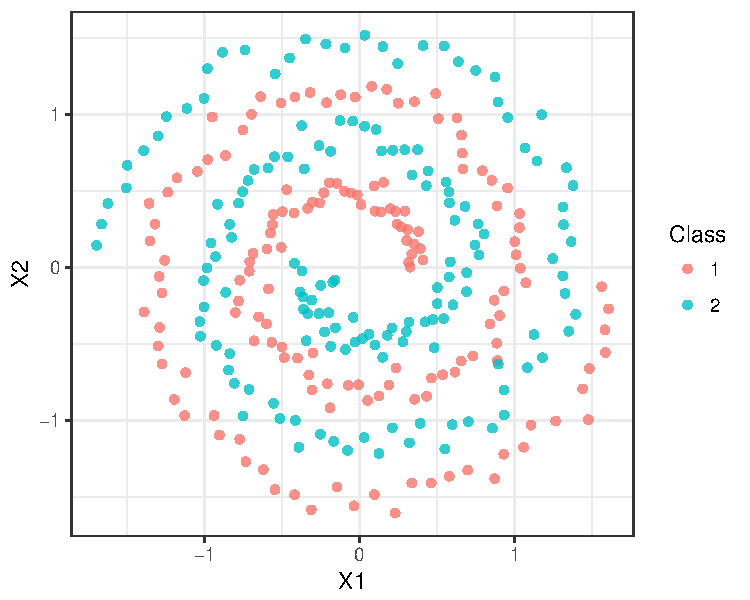
\includegraphics[width=0.7\linewidth]{figure/spiral_data-1} 

}

\caption[Spiral data set]{Spiral data set.}\label{fig:spiral_data}
\end{figure}


\end{knitrout}

We tried a few models. First with the linear canonical kernel. This gave very poor results (training error rate of 50\% is basically just guess-work). Not surprising because the problem hardly seems linear in nature. Best to go with a smooth function, so we tried the fBm kernel. This gave an improved training error rate (31.3\%) but judging by the predictive plot, there still is room for improvement.

\begin{knitrout}
\definecolor{shadecolor}{rgb}{1, 1, 1}\color{fgcolor}\begin{kframe}
\begin{alltt}
\hlstd{R> }\hlcom{# Bad results, linear functions not able to predict spirals well}
\hlstd{R> }\hlstd{(mod1} \hlkwb{<-} \hlkwd{iprobit}\hlstd{(y} \hlopt{~} \hlstd{X1} \hlopt{+} \hlstd{X2, spiral,} \hlkwc{kernel} \hlstd{=} \hlstr{"Canonical"}\hlstd{))}
\end{alltt}
\begin{verbatim}
## ===========
## Converged after 15 iterations.
## Training error rate: 50.00 %
## Lower bound value: -214.0725 
## 
##     alpha lambda[1] lambda[2] 
##   0.00004   0.00000   2.88634
\end{verbatim}
\begin{alltt}
\hlstd{R> }\hlkwd{iplot_predict}\hlstd{(mod1)}
\end{alltt}
\end{kframe}\begin{figure}[h]

{\centering 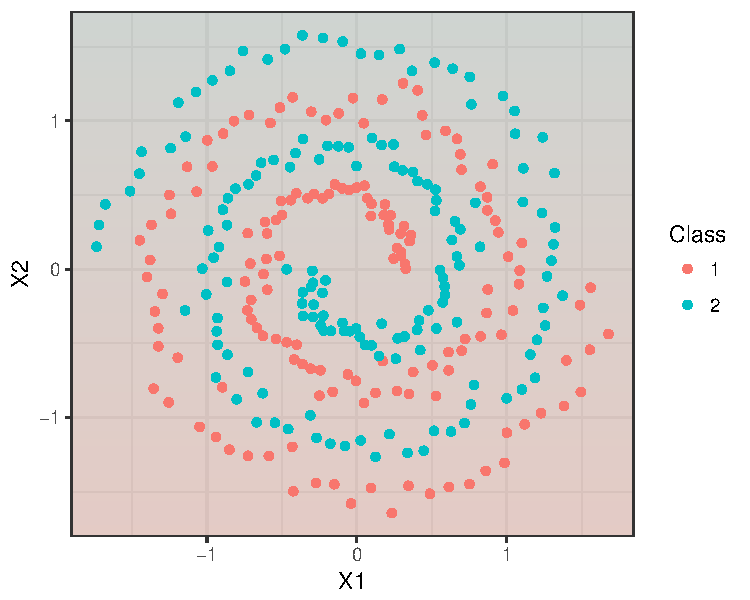
\includegraphics[width=0.7\linewidth]{figure/spiral_canonical-1} 

}

\caption[Canonical kernel with multiple scale parameters]{Canonical kernel with multiple scale parameters.}\label{fig:spiral_canonical}
\end{figure}


\end{knitrout}

\begin{knitrout}
\definecolor{shadecolor}{rgb}{1, 1, 1}\color{fgcolor}\begin{kframe}
\begin{alltt}
\hlstd{R> }\hlcom{# Getting there, but still not nice}
\hlstd{R> }\hlstd{(mod2} \hlkwb{<-} \hlkwd{iprobit}\hlstd{(y} \hlopt{~} \hlstd{X1} \hlopt{+} \hlstd{X2, spiral,} \hlkwc{kernel} \hlstd{=} \hlstr{"FBM"}\hlstd{))}
\end{alltt}
\begin{verbatim}
## ======================================================================
## Convergence criterion not met.
## Training error rate: 31.33 %
## Lower bound value: -204.2227 
## 
##     alpha lambda[1] lambda[2] 
##   0.00484  -0.00263   1.26369
\end{verbatim}
\begin{alltt}
\hlstd{R> }\hlkwd{iplot_predict}\hlstd{(mod2)}
\end{alltt}
\end{kframe}\begin{figure}[h]

{\centering 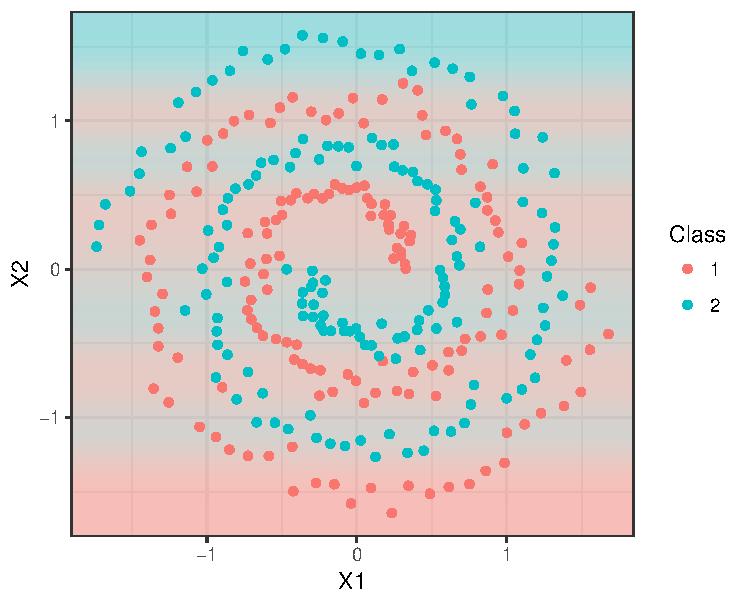
\includegraphics[width=0.7\linewidth]{figure/spiral_fbm-1} 

}

\caption[fBm kernel with multiple scale parameters]{fBm kernel with multiple scale parameters.}\label{fig:spiral_fbm}
\end{figure}


\end{knitrout}

\begin{knitrout}
\definecolor{shadecolor}{rgb}{1, 1, 1}\color{fgcolor}\begin{kframe}
\begin{alltt}
\hlstd{R> }\hlcom{# Turns out the scale parameters matter here}
\hlstd{R> }\hlstd{(mod3} \hlkwb{<-} \hlkwd{iprobit}\hlstd{(y} \hlopt{~} \hlstd{X1} \hlopt{+} \hlstd{X2, spiral,} \hlkwc{kernel} \hlstd{=} \hlstr{"FBM"}\hlstd{,} \hlkwc{one.lam} \hlstd{=} \hlnum{TRUE}\hlstd{))}
\end{alltt}
\begin{verbatim}
## ==========================================================
## Converged after 82 iterations.
## Training error rate: 1.67 %
## Lower bound value: -162.9976 
## 
##   alpha  lambda 
## 0.00497 5.16273
\end{verbatim}
\begin{alltt}
\hlstd{R> }\hlkwd{iplot_predict}\hlstd{(mod3)}
\end{alltt}
\end{kframe}\begin{figure}[h]

{\centering 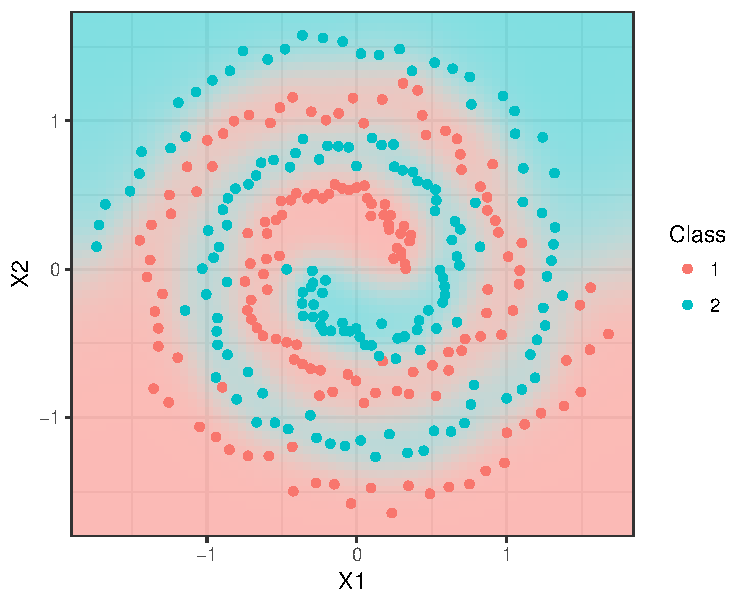
\includegraphics[width=0.7\linewidth]{figure/spiral_fbm_onelam-1} 

}

\caption[fBm kernel with a single shared scale parameter]{fBm kernel with a single shared scale parameter.}\label{fig:spiral_fbm_onelam}
\end{figure}


\end{knitrout}

It turns out that retstricting the model to have a single scale parameter works best, coupled with the fBm kernel. This seems to suggest that the two variables are similarly scaled and effects the latent response in a similar magnitude. Indeed, the $X_1$ and $X_2$ variables are quite similar in that they are points from two spirals mirroring each other. We are able to get a training error rate of 1.67\%, and incidentally this model gives the highest lower-bound value as well.

One thing that was noticed with this data set was that different starting values led to possibly different converged parameter estimates. This leads us to believe that the variational lower bound to be maximised has multiple local optima. One way to overcome this is to perform multiple restarts and keep the results from the highest lower bound value. This is something to look out for when analysing real-data examples.

The next example is a four-class classification data set that is meant to be linearly separable in two dimensions. Random noise was added to the $X_1$ and $X_2$ component from four equidistant points (representing four distinct classes) around a circle of radius three. 125 points were generated for each class, thereby giving a total of 500 data points altogether. Here is a plot of the data set.

\begin{knitrout}
\definecolor{shadecolor}{rgb}{1, 1, 1}\color{fgcolor}\begin{kframe}
\begin{alltt}
\hlstd{R> }\hlstd{mixture} \hlkwb{<-} \hlkwd{gen_mixture}\hlstd{(}\hlkwc{n} \hlstd{=} \hlnum{500}\hlstd{,} \hlkwc{m} \hlstd{=} \hlnum{4}\hlstd{,} \hlkwc{sd} \hlstd{=} \hlnum{1.5}\hlstd{)}
\hlstd{R> }\hlstd{(mod} \hlkwb{<-} \hlkwd{iprobit}\hlstd{(y} \hlopt{~} \hlstd{X1} \hlopt{+} \hlstd{X2, mixture))}
\end{alltt}
\begin{verbatim}
## ======================================================================
## Convergence criterion not met.
## Training error rate: 8.80 %
## Lower bound value: -194.2465 
## 
##            Class = 1 Class = 2 Class = 3 Class = 4
## alpha       -0.12285  -0.71550  -0.72534  -0.07966
## lambda[1,]   1.28355   0.00000   0.70112   0.00000
## lambda[2,]   0.00000   0.25543   0.00000   1.02738
\end{verbatim}
\end{kframe}
\end{knitrout}

We fit a canonical I-probit model, and get the following results.

\begin{knitrout}
\definecolor{shadecolor}{rgb}{1, 1, 1}\color{fgcolor}\begin{kframe}
\begin{alltt}
\hlstd{R> }\hlkwd{plot}\hlstd{(mixture)}
\hlstd{R> }\hlkwd{iplot_predict}\hlstd{(mod)}
\end{alltt}
\end{kframe}\begin{figure}[h]

{\centering 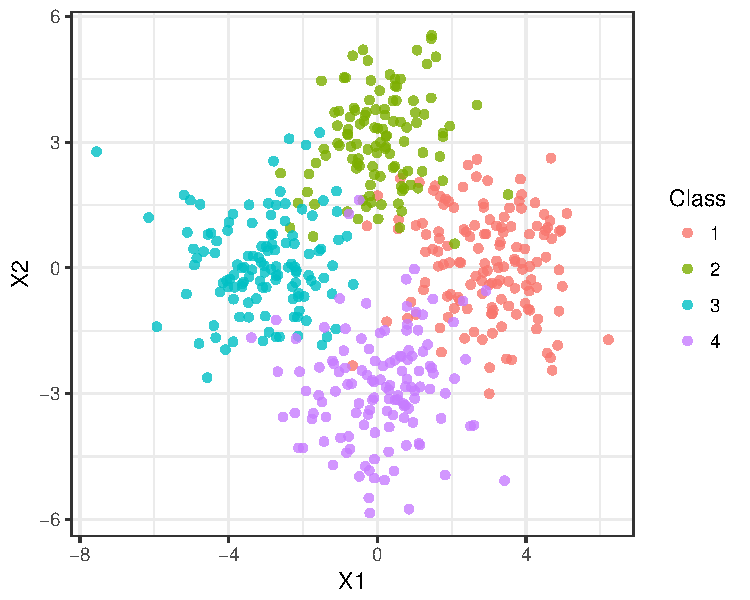
\includegraphics[width=0.49\linewidth]{figure/mixture_mod_plot-1} 
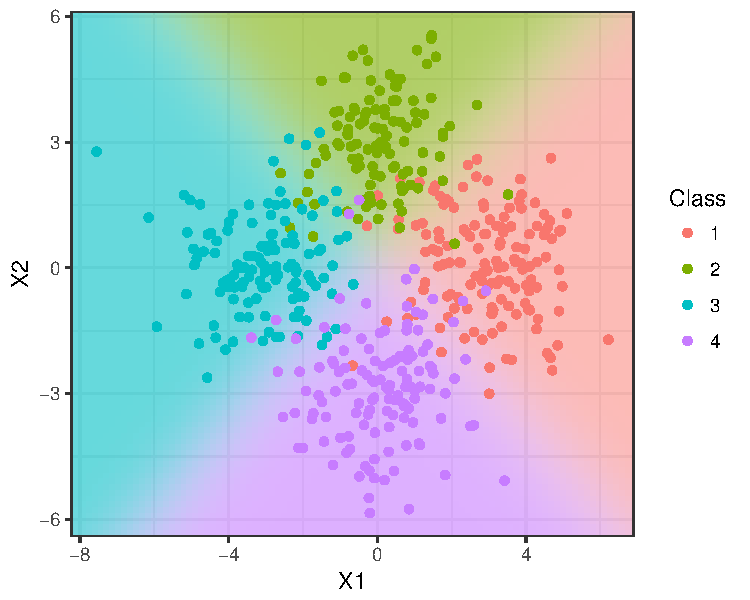
\includegraphics[width=0.49\linewidth]{figure/mixture_mod_plot-2} 

}

\caption[Canonical kernel is able to linearly separate the data points]{Canonical kernel is able to linearly separate the data points.}\label{fig:mixture_mod_plot}
\end{figure}


\end{knitrout}

\end{document}




\section{Predicting cardiac arrhythmia}
\documentclass[a4paper,showframe,11pt]{report}\usepackage[]{graphicx}\usepackage[]{color}
%% maxwidth is the original width if it is less than linewidth
%% otherwise use linewidth (to make sure the graphics do not exceed the margin)
\makeatletter
\def\maxwidth{ %
  \ifdim\Gin@nat@width>\linewidth
    \linewidth
  \else
    \Gin@nat@width
  \fi
}
\makeatother

\definecolor{fgcolor}{rgb}{0.196, 0.196, 0.196}
\newcommand{\hlnum}[1]{\textcolor[rgb]{0.063,0.58,0.627}{#1}}%
\newcommand{\hlstr}[1]{\textcolor[rgb]{0.063,0.58,0.627}{#1}}%
\newcommand{\hlcom}[1]{\textcolor[rgb]{0.588,0.588,0.588}{#1}}%
\newcommand{\hlopt}[1]{\textcolor[rgb]{0.196,0.196,0.196}{#1}}%
\newcommand{\hlstd}[1]{\textcolor[rgb]{0.196,0.196,0.196}{#1}}%
\newcommand{\hlkwa}[1]{\textcolor[rgb]{0.231,0.416,0.784}{#1}}%
\newcommand{\hlkwb}[1]{\textcolor[rgb]{0.627,0,0.314}{#1}}%
\newcommand{\hlkwc}[1]{\textcolor[rgb]{0,0.631,0.314}{#1}}%
\newcommand{\hlkwd}[1]{\textcolor[rgb]{0.78,0.227,0.412}{#1}}%
\let\hlipl\hlkwb

\usepackage{framed}
\makeatletter
\newenvironment{kframe}{%
 \def\at@end@of@kframe{}%
 \ifinner\ifhmode%
  \def\at@end@of@kframe{\end{minipage}}%
  \begin{minipage}{\columnwidth}%
 \fi\fi%
 \def\FrameCommand##1{\hskip\@totalleftmargin \hskip-\fboxsep
 \colorbox{shadecolor}{##1}\hskip-\fboxsep
     % There is no \\@totalrightmargin, so:
     \hskip-\linewidth \hskip-\@totalleftmargin \hskip\columnwidth}%
 \MakeFramed {\advance\hsize-\width
   \@totalleftmargin\z@ \linewidth\hsize
   \@setminipage}}%
 {\par\unskip\endMakeFramed%
 \at@end@of@kframe}
\makeatother

\definecolor{shadecolor}{rgb}{.97, .97, .97}
\definecolor{messagecolor}{rgb}{0, 0, 0}
\definecolor{warningcolor}{rgb}{1, 0, 1}
\definecolor{errorcolor}{rgb}{1, 0, 0}
\newenvironment{knitrout}{}{} % an empty environment to be redefined in TeX

\usepackage{alltt}
\usepackage{standalone}
\standalonetrue
\ifstandalone
  \usepackage{../../haziq_thesis}
  \usepackage{../../haziq_maths}
  \usepackage{../../haziq_glossary}
  \addbibresource{../../bib/haziq.bib}
  \externaldocument{../01/.texpadtmp/introduction}
\fi





\IfFileExists{upquote.sty}{\usepackage{upquote}}{}
\begin{document}

Machine learning tools are being used in the field of medicine as a means to aid medical diagnosis of diseases. In this example, factors determining the presence or absence of heart diseses is studied. Traditionally, cardiologists may look at patients' cardiac activity (ECG data) to reach a diagnosis. This of course remains the so-called ``gold standard'' method of obtaining a diagnosis. The study by Guvenir et. al. aimed to predict cardiac abnormalities by way of machine learning and minimise the difference between the gold standard and computer-based classifications. This data set is made publicly available at [...]. It contains a myriad of ECG readings and other patient attributes such as age, height, and weight. Altogether there are 451 observations and 279 predictors. We excluded nominal covariates, leaving us with 194 continuous predictors, which we then standardised so that we can use a single-scale I-probit model. In the original data set, there are 13 distinct classes of cardiac arrhythmia. We had combined all of these to form a single class, thus reducing the problem to a binary classification task (normal vs. arrhythmia).

Fitting an I-probit model on the full data set takes about 2.5 seconds only, with convergence reached in at most 15 iterations.
However, we do find that the training error rates are much better if the model was not allowed to reach full convergence (i.e., stopped early at five iterations, say)
\hltodo{Why is this? Need to look at a plot of marginal likelihood.}.
It is believed that local optima gives better predictive performance, rather than at the global maxima of the (approximate) likelihood.

Figure \ref{fig:cardiac.mod.full.plot}(a) plots the variational lower bound value over time and iterations for the cardiac arrhythmia data set. As expected, the lower bound value increases over time until a convergence criterion is reached. In Figure \ref{fig:cardiac.mod.full.plot}(b), the training error rate and the Brier score is plotted against time. What we see is that the training error rate worsens over time as the lower bound value reaches its maximum value. There is some reason to terminate the variational algorithm early - while compromising on the lower bound value, we hope to obtain parameter values which give good predictive performance.


\begin{knitrout}
\definecolor{shadecolor}{rgb}{1, 1, 1}\color{fgcolor}\begin{figure}

{\centering 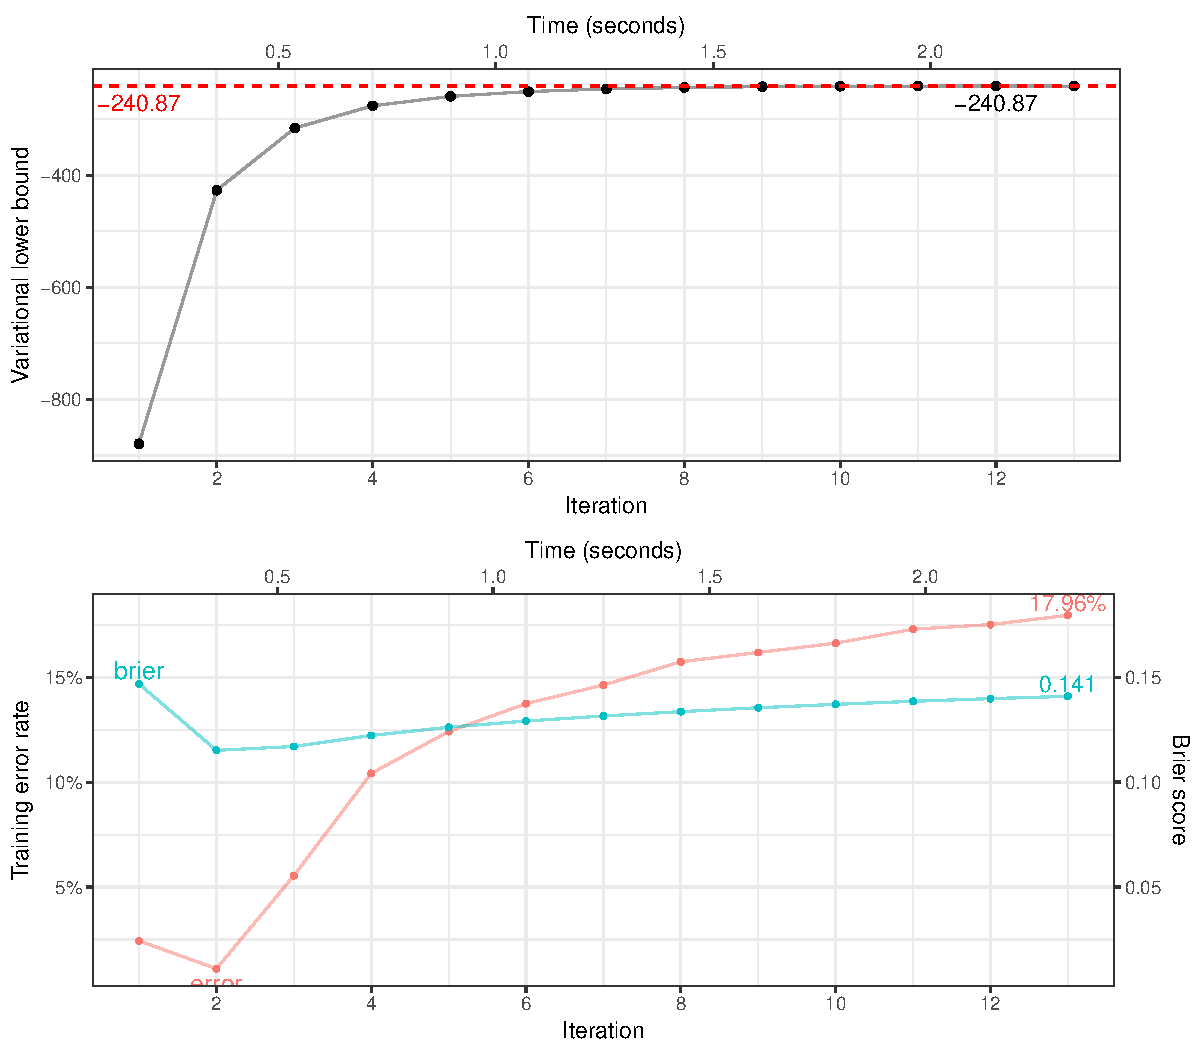
\includegraphics[width=\linewidth]{figure/cardiac_mod_full_plot-1} 

}

\caption[(a) Plot of variational lower bound over time]{(a) Plot of variational lower bound over time. (b) Plot of training error rate and Brier scores over time.}\label{fig:cardiac.mod.full.plot}
\end{figure}


\end{knitrout}

To measure predictive ability, we fit the I-probit model with the canonical and fBm-0.5 kernel on a random subset of the data and obtain the out-of-sample test error rates from the remaining observations. We then compare the results against popular machine learning classifiers, namely: 1) $k$-nearest neighbours; 2) support vector machine; 3) Gaussian process classification (radial basis kernel); 4) random forests; 5) nearest shrunken centroids (Tibshirani et. al. 2003); and 6) L-1 penalised logistic regression. The final model also performs variable selection, something that the I-probit model can do as well, but for now we concentrate on using all the available predictors for training and testing. The experiment is set up as follows:
\begin{enumerate}
  \item Form a training set by sub-sampling $n \in \{50, 100, 200\}$ observations.
  \item The remaining unsampled data is used as the test set.
  \item Fit model on training set, and obtain test error rates defined as
  \[
    \text{test error rate} = \frac{1}{n} \sum_{i=1}^n [y^{\text{pred}}_i \neq y^{\text{test}}_i] \times 100 \%.
  \]
  \item Repeat steps 1-3 100 times to obtain the \emph{average} test error rates and standard errors.
\end{enumerate}
Results for the six methods listed above were obtained from Cannings and Samworth (2017). The results are shown in the plot below.


\begin{knitrout}
\definecolor{shadecolor}{rgb}{1, 1, 1}\color{fgcolor}\begin{figure}

{\centering 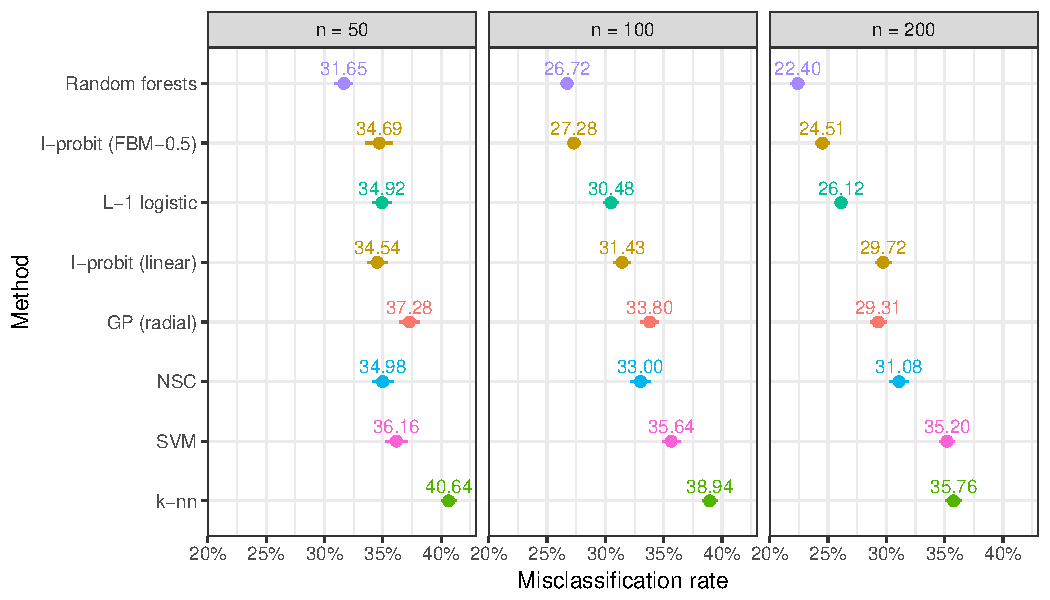
\includegraphics[width=\maxwidth]{figure/plot_cardiac-1} 

}

\caption[Plot of mean test error rates (points) together with the 95\% confidence intervals for I-probit models and six popular classifiers]{Plot of mean test error rates (points) together with the 95\% confidence intervals for I-probit models and six popular classifiers.}\label{fig:plot_cardiac}
\end{figure}


\end{knitrout}

A plot of the mean test error rates together with the 95\% confidence intervals for all models are shown in Figure \ref{fig:plot_cardiac}. The methods shown in the plot are sorted from the best (top) to the worst (bottom), according to a weighted ranking system which favours better performance in smaller sub-samples. It can be seen that the I-probit models outperform the more popular machine learning algorithms out there including $k$-nearest neighbours, support vector machines and Gaussian process classification. The fBm I-probit model performed better than the canonical linear I-probit model, which is unsurprising. An underlying smooth function to model the latent variables is expected to generalise better than a rigid straight line function. The fBm I-probit model came second only to random forests, an ensemble learning method, which depending on the number of random decisions trees generated simultaneously, might be slow. The time complexity of a random forest algorithm is $O(pqn\log(n))$, where $p$ is the number of variables used for training, $q$ is the number of random decision trees, and $n$ is the number of observations.

\end{document}




\section{Meta-analysis of smoking cessation}
\documentclass[a4paper,showframe,11pt]{report}\usepackage[]{graphicx}\usepackage[]{color}
%% maxwidth is the original width if it is less than linewidth
%% otherwise use linewidth (to make sure the graphics do not exceed the margin)
\makeatletter
\def\maxwidth{ %
  \ifdim\Gin@nat@width>\linewidth
    \linewidth
  \else
    \Gin@nat@width
  \fi
}
\makeatother

\definecolor{fgcolor}{rgb}{0.196, 0.196, 0.196}
\newcommand{\hlnum}[1]{\textcolor[rgb]{0.063,0.58,0.627}{#1}}%
\newcommand{\hlstr}[1]{\textcolor[rgb]{0.063,0.58,0.627}{#1}}%
\newcommand{\hlcom}[1]{\textcolor[rgb]{0.588,0.588,0.588}{#1}}%
\newcommand{\hlopt}[1]{\textcolor[rgb]{0.196,0.196,0.196}{#1}}%
\newcommand{\hlstd}[1]{\textcolor[rgb]{0.196,0.196,0.196}{#1}}%
\newcommand{\hlkwa}[1]{\textcolor[rgb]{0.231,0.416,0.784}{#1}}%
\newcommand{\hlkwb}[1]{\textcolor[rgb]{0.627,0,0.314}{#1}}%
\newcommand{\hlkwc}[1]{\textcolor[rgb]{0,0.631,0.314}{#1}}%
\newcommand{\hlkwd}[1]{\textcolor[rgb]{0.78,0.227,0.412}{#1}}%
\let\hlipl\hlkwb

\usepackage{framed}
\makeatletter
\newenvironment{kframe}{%
 \def\at@end@of@kframe{}%
 \ifinner\ifhmode%
  \def\at@end@of@kframe{\end{minipage}}%
  \begin{minipage}{\columnwidth}%
 \fi\fi%
 \def\FrameCommand##1{\hskip\@totalleftmargin \hskip-\fboxsep
 \colorbox{shadecolor}{##1}\hskip-\fboxsep
     % There is no \\@totalrightmargin, so:
     \hskip-\linewidth \hskip-\@totalleftmargin \hskip\columnwidth}%
 \MakeFramed {\advance\hsize-\width
   \@totalleftmargin\z@ \linewidth\hsize
   \@setminipage}}%
 {\par\unskip\endMakeFramed%
 \at@end@of@kframe}
\makeatother

\definecolor{shadecolor}{rgb}{.97, .97, .97}
\definecolor{messagecolor}{rgb}{0, 0, 0}
\definecolor{warningcolor}{rgb}{1, 0, 1}
\definecolor{errorcolor}{rgb}{1, 0, 0}
\newenvironment{knitrout}{}{} % an empty environment to be redefined in TeX

\usepackage{alltt}
\usepackage{standalone}
\standalonetrue
\ifstandalone
  \usepackage{../../haziq_thesis}
  \usepackage{../../haziq_maths}
  \usepackage{../../haziq_glossary}
  \addbibresource{../../bib/haziq.bib}
  \externaldocument{../01/.texpadtmp/introduction}
\fi





\IfFileExists{upquote.sty}{\usepackage{upquote}}{}
\begin{document}

Data from 27 separate smoking cessation studies in which participants are subjected to a nicotine gum treatment or a placebo.
The interest is to estimate the treatment effect size, and whether it is statistically significant.
The studies are conducted at different times and due to various reasons such as funding and cultural effects, the results from all of the studies may not be in agreement.
The number of effective participants plays a major role in determining the power of the statistical tests performed in individual studies.
The question then becomes how do we meaningfully aggregate all the data to come up with one summary measure?

Several methods exist to analyse such data sets.
One may consider a fixed-effects model, similar to a one-way ANOVA model to establish whether or not the effect size is significant.
Because of the study-specific characteristics, it is natural to consider multilevel or random-effects models as a means to estimate the effect size.
Regardless of method, the approach of analysing study-level treatment effects instead of patient-level data is the paradigm for meta-analysis.
However, analysing study-level estimates of effect size can be problematic for various reasons, such as small group samples or rare occurences.
Our approach using I-priors looks at patient-level data, but takes into account the levels due to the various study groups.

\begin{knitrout}
\definecolor{shadecolor}{rgb}{1, 1, 1}\color{fgcolor}\begin{figure}

{\centering 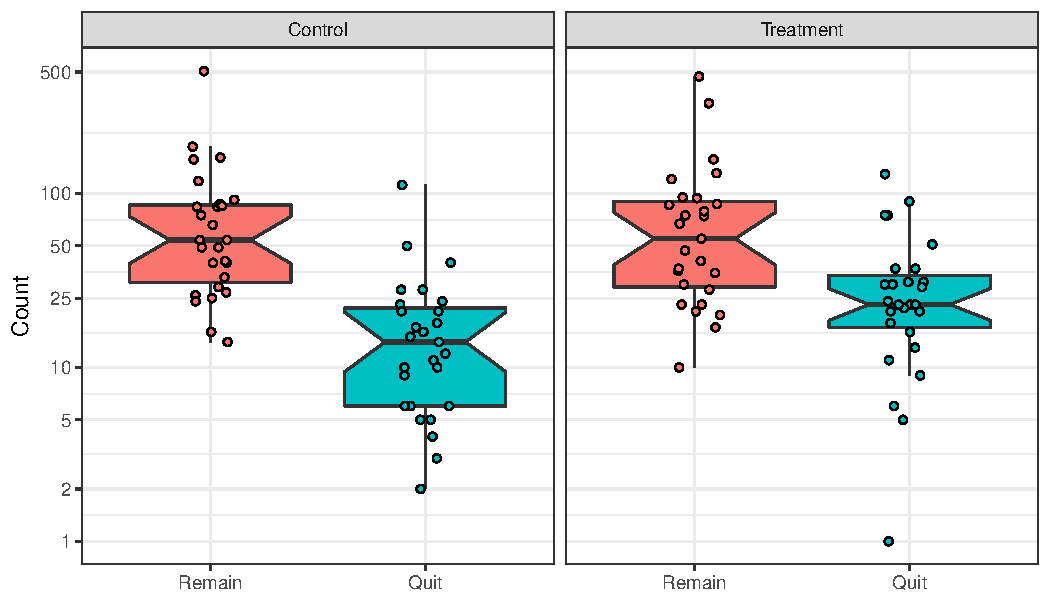
\includegraphics[width=\maxwidth]{figure/plot_data_smoke-1} 

}

\caption[Comparative box-plots of the distribution of patients who successfully quit smoking and those who remained smokers, in the two treatment groups]{Comparative box-plots of the distribution of patients who successfully quit smoking and those who remained smokers, in the two treatment groups.}\label{fig:plot.data.smoke}
\end{figure}


\end{knitrout}

A summary of the data is displayed by the box-plot in Figure \ref{fig:plot.data.smoke}.
On the whole, there are a total of 5908 patients, and they are distributed roughly equally among the control and treatment groups (46.33\% and 53.67\% respectively, on average).
From the box-plots, it is evident that there are more patients who quit smoking in the treatment group as compared to the placebo control group.
There are various measures of treatment effect size, such as risk ratio or risk differences, but we shall concentrate on \emph{odds ratios} as defined by
\[
  \text{odds ratio} = \frac{\text{odds of quitting smoking in \emph{treatment} group}}
  {\text{odds of quitting smoking in \emph{control} group}}.
\]
The odds of quitting smoking in either group is defined as
\[
  \text{odds} = \frac{\Prob[\text{quit smoking}]}{1 - \Prob[\text{quit smoking}]},
\]
and these probabilities, odds and ultimately the odds ratio can be estimated from sample proportions.
This raw odds ratio for all study groups is calculated as $1.66 = e^{0.50}$.
It is also common for the odds ratio to be reported on the log scale (usually as a remnant of logistic models).
A value greater than one for the odds ratio (or equivalently, greater than zero for the log-odds ratio) indicates a significant treatment effect.

A random-effects analysis using a multilevel logistic model has been considered by \hltodo{cite Skrondal Rabe-Hasketh, Agresti and Hartzel}.
Let $i=1,\dots,n_j$ index the patients in study group $j \in \{1,\dots,27\}$.
For patient $i$ in study $j$, $p_{ij}$ denotes the probability that the patient has successfully quit smoking.
Additionally, $x_{ij}$ is the centred dummy variable indicating patient $i$'s treatment group in study $j$.
These take on two values: 0.5 for treated patients and -0.5 for control patients.
The logistic random-effects model is
\begin{gather*}
  \log \left( \frac{p_{ij}}{1-p_{ij}} \right) = \beta_{0j} + \beta_{1j}x_{ij} \\
  \text{with} \\
  \begin{pmatrix} \beta_{0j} \\ \beta_{1j} \end{pmatrix}
  \sim \N \left(
  \begin{pmatrix} \beta_0 \\ \beta_1 \end{pmatrix},
  \begin{pmatrix} \sigma_0^2 & \sigma_{01} \\ \sigma_{01} & \sigma_1^2 \\ \end{pmatrix}
  \right)
\end{gather*}
Agresti also made the additional assumption that $\sigma_{01} = 0$ so that, coupled with the contrast coding used for $x_{ij}$, the total variance $\Var[\beta_{0j} + \beta_{1j}x_{ij}]$ would be constant in both treatment groups.
The overall log odds ratio is represented by $\beta_1$, and this is estimated as $0.57 = \log 1.76$.

In an I-prior model, the Bernoulli probabilities $p_{ij}$ are regressed against the treatment group indicators $x_{ij}$ and also the patients' study group $j$ via the regression function $f$ and a probit link:
\begin{align*}
  \Phi^{-1}(p_{ij})
  &= f(x_{ij}, j) \\
  &= f_1(x_{ij}) + f_2(j) + f_{12}(x_{ij}, j).
\end{align*}
We have decomposed our function $f$ into three parts: $f_1$ represents the treatment effect, $f_2$ represents the effect of the study groups, and $f_{12}$ represents the interaction effect between the treatment and study group on the modelled probabilities.
As both $x_{ij}$ and $j$ are nominal variables, the functions $f_1$ and $f_2$ both lie in the Pearson RKHS of functions $\cF_1$ and $\cF_2$, each with RKHS scale parameters $\lambda_1$ and $\lambda_2$.
As such, it does not matter how the $x_{ij}$ variables are coded (dummy coding 0, 1 vs. centred coding -0.5, 0.5) as the scaling of the function is determined by the RKHS scale parameters.
The interaction effect $f_{12}$ lies in the RKHS tensor product $\cF_1 \otimes \cF_2$.
In I-prior modelling, there are only two parameters to estimate, while in the standard logistic random-effects model, there are six. The results of the I-prior fit are summarised in the table below.


\begin{longtable}[t]{lrr>{\raggedleft\arraybackslash}p{2.4cm}}
\caption{\label{tab:mod.compare.smoke}Results of the I-prior model fit for three models.}\\
\toprule
Model & Lower bound & Brier score & No. of RKHS\newline scale param.\\
\midrule
$f_1$ & $-3210.76$ & 0.179 & 1\\
$f_1 + f_2$ & $-3092.22$ & 0.168 & 2\\
$f_1 + f_2 + f_{12}$ & $-3091.21$ & 0.168 & 2\\
\bottomrule
\end{longtable}



The approximated marginal log-likelihood value for the I-prior model (i.e. variational lower bound), the Brier score for each model and the number of RKHS scale parameters estimated in the model are reported in Table \ref{tab:mod.compare.smoke}. Three models were fitted: : 1) A model with only the treatment effect; 2) A model with a treatment effect and a study group effect; and 3) Model 2 with the additional assumption that treatment effect varies across study groups. Model 1 disregards the study group effects, while Model 2 assumes that the effectiveness of the nicotine gum treatment does not vary across study groups (akin to a varying-intercept model). Although not soundly based in theory, we may compare variational lower bounds of the three models for model selection as a proxy to using the true log-likelihood value. In this case, Model 3 has the highest lower bound value. The Brier score indicates the predictive performance of the models, and there is not much to distinguish between the three.

Unlike in the logistic random-effects model, where the log odds ratio can be read off directly from the coefficients, with an I-prior probit model the log odds ratio needs to be calculated manually from the fitted probabilities. The probabilities of interest are the probabilities of quitting smoking under each treatment group for each study group $j$ - call these $p_j(\text{treatment})$ and $p_j(\text{control})$. That is,
\begin{align*}
  p_j(\text{treatment}) &= \Phi\big( f(\text{treatment}, j) \big) \\
  p_j(\text{control})   &= \Phi\big( f(\text{control}, j) \big). \\
\end{align*}
The log odds ratio for each study group can then be calculated as usual.
For the overall log odds ratio, the probabilities that are used are the averaged probabilities weighted according to the sample sizes in each group. This has been calculated as $0.50 = \log 1.64$, slightly lower than both the raw log odds ratio and the log odds ratio estimated by the logistic random-effects model. This can perhaps be attributed to some shrinkage of the estimated probabilities due to placing a prior with zero mean on the regression functions.

\hltodo{RE: Fiona's suggestion of discussing the variance, covariance/correlation of the random effects?}

\begin{knitrout}
\definecolor{shadecolor}{rgb}{1, 1, 1}\color{fgcolor}\begin{figure}

{\centering 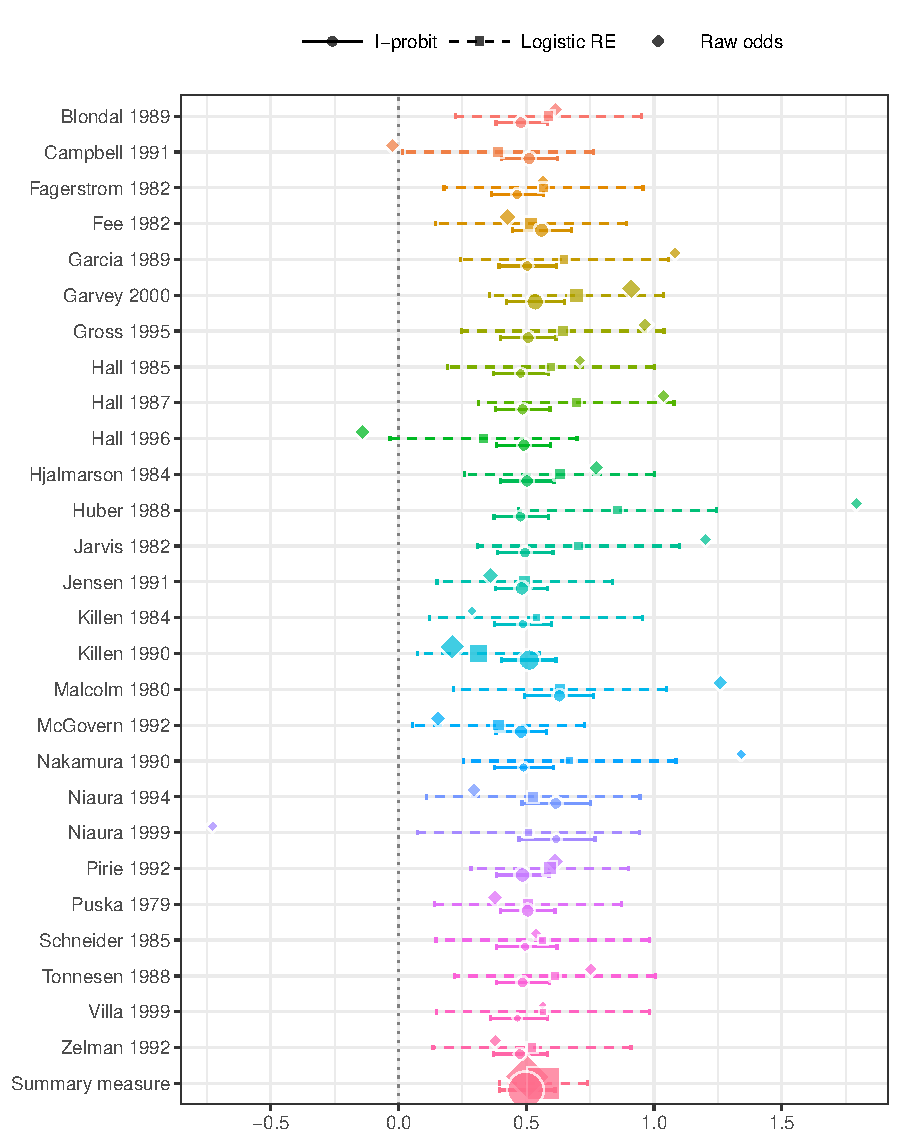
\includegraphics[width=\linewidth]{figure/smoke_forest_plot-1} 

}

\caption[Forest plot of effect sizes (log odds ratios) in each group as well as the overall effect size together with their 95\% confidence bands]{Forest plot of effect sizes (log odds ratios) in each group as well as the overall effect size together with their 95\% confidence bands. The plot compares the raw log odds ratios, the logistic random-effect estimates, and the I-prior estimates. Sizes of the points indicate the relative sample sizes per study group.}\label{fig:smoke.forest.plot}
\end{figure}


\end{knitrout}

\end{document}




\section{Vowel recognition data}
\documentclass[a4paper,showframe,11pt]{report}\usepackage[]{graphicx}\usepackage[]{color}
%% maxwidth is the original width if it is less than linewidth
%% otherwise use linewidth (to make sure the graphics do not exceed the margin)
\makeatletter
\def\maxwidth{ %
  \ifdim\Gin@nat@width>\linewidth
    \linewidth
  \else
    \Gin@nat@width
  \fi
}
\makeatother

\definecolor{fgcolor}{rgb}{0.196, 0.196, 0.196}
\newcommand{\hlnum}[1]{\textcolor[rgb]{0.063,0.58,0.627}{#1}}%
\newcommand{\hlstr}[1]{\textcolor[rgb]{0.063,0.58,0.627}{#1}}%
\newcommand{\hlcom}[1]{\textcolor[rgb]{0.588,0.588,0.588}{#1}}%
\newcommand{\hlopt}[1]{\textcolor[rgb]{0.196,0.196,0.196}{#1}}%
\newcommand{\hlstd}[1]{\textcolor[rgb]{0.196,0.196,0.196}{#1}}%
\newcommand{\hlkwa}[1]{\textcolor[rgb]{0.231,0.416,0.784}{#1}}%
\newcommand{\hlkwb}[1]{\textcolor[rgb]{0.627,0,0.314}{#1}}%
\newcommand{\hlkwc}[1]{\textcolor[rgb]{0,0.631,0.314}{#1}}%
\newcommand{\hlkwd}[1]{\textcolor[rgb]{0.78,0.227,0.412}{#1}}%
\let\hlipl\hlkwb

\usepackage{framed}
\makeatletter
\newenvironment{kframe}{%
 \def\at@end@of@kframe{}%
 \ifinner\ifhmode%
  \def\at@end@of@kframe{\end{minipage}}%
  \begin{minipage}{\columnwidth}%
 \fi\fi%
 \def\FrameCommand##1{\hskip\@totalleftmargin \hskip-\fboxsep
 \colorbox{shadecolor}{##1}\hskip-\fboxsep
     % There is no \\@totalrightmargin, so:
     \hskip-\linewidth \hskip-\@totalleftmargin \hskip\columnwidth}%
 \MakeFramed {\advance\hsize-\width
   \@totalleftmargin\z@ \linewidth\hsize
   \@setminipage}}%
 {\par\unskip\endMakeFramed%
 \at@end@of@kframe}
\makeatother

\definecolor{shadecolor}{rgb}{.97, .97, .97}
\definecolor{messagecolor}{rgb}{0, 0, 0}
\definecolor{warningcolor}{rgb}{1, 0, 1}
\definecolor{errorcolor}{rgb}{1, 0, 0}
\newenvironment{knitrout}{}{} % an empty environment to be redefined in TeX

\usepackage{alltt}
\usepackage{standalone}
\standalonetrue
\ifstandalone
  \usepackage{../../haziq_thesis}
  \usepackage{../../haziq_maths}
  \usepackage{../../haziq_glossary}
  \addbibresource{../../bib/haziq.bib}
  \externaldocument{../01/.texpadtmp/introduction}
\fi







\IfFileExists{upquote.sty}{\usepackage{upquote}}{}
\begin{document}

\hltodo{cite Hastie Tibshirani elements of statistical learning}.
We illustrate multiclass classification using I-priors on a speech recognition data set\footnotemark with $m = 11$ classes to be predicted from digitized low pass filtered signals generated from voice recordings.
Each class corresponds to a vowel sound made when pronouncing a specific word.
The words that make up the vowel sounds are shown in Table \ref{tab:vowel}. Each word was uttered once by multiple speakers, and the data are split into a training and a test set.
Four males and four female speakers contributed to the training set, while four male and three female speakers contributed to the test set.
The recordings were manipulated using speech processing techniques, such that each speaker yielded six frames of speech from the eleven vowels, each with a corresponding 10-dimensional numerical input vector (the predictors).
This means that the size of the training set is 528, while 462 data points are available for testing the predictive performance of the models.
This data set is also known as Deterding's vowel recognition data (after the original collector, cite) or the Connectionist Bench data.
Machine learning methods such as neural networks and nearest neighbour methods were analysed by Robinson (cite).

\footnotetext{Data is publicaly available from the UCI Machine Learning Repository, URL: \url{https://archive.ics.uci.edu/ml/datasets/Connectionist+Bench+(Vowel+Recognition+-+Deterding+Data)}.}

\begin{table}[]
\centering
\caption{The eleven words that make up the classes of vowels.}
\label{tab:vowel}
\begin{tabular}{llllllllll}
\toprule
Class & Label          & Vowel & Word &  && Class & Label          & Vowel & Word  \\
\midrule
1     & \texttt{hid} & \dsil{iː}    & heed &&  & 7     & \texttt{hOd} & \dsil{ɒ}    & hod   \\
2     & \texttt{hId} & \dsil{ɪ}     & hid  &&  & 8     & \texttt{hod} & \dsil{ɔː}   & hoard \\
3     & \texttt{hEd} & \dsil{ɛ}     & head &&  & 9     & \texttt{hUd} & \dsil{ʊ}    & hood  \\
4     & \texttt{hAd} & \dsil{a}     & had  &&  & 10    & \texttt{hud} & \dsil{uː}   & who'd \\
5     & \texttt{hYd} & \dsil{ʌ}     & hud  &&  & 11    & \texttt{hed} & \dsil{əː}   & heard \\
6     & \texttt{had} & \dsil{ɑː}    & hard &&  &       &              &             &       \\
\bottomrule
\end{tabular}
\end{table}

We will fit the data using an I-probit model with the canonical linear kernel and also the fBm-0.5 kernel.
We assume $m = 11$ distinct I-priors corresponding to the latent variables in each class, thus there are 11 unique intercepts and 11 RKHS scale parameters to estimate in each model.
Each model took roughly 6 seconds per iteration to complete.
The canonical kernel model took a long time to converge, with each variational EM iteration improving the lower bound only slighly each time.
In contrast, the fBm-0.5 model was quicker to converge, and this is something that we noticed happening for most other data sets as well.
Multiple restarts from different random seeds were conducted, and we found that they all converged to a similar lower bound value.
This alleviates any worry that the model might have converged to different multiple local optima.

\begin{knitrout}
\definecolor{shadecolor}{rgb}{1, 1, 1}\color{fgcolor}\begin{figure}[h]

{\centering \subfloat[Canonical kernel\label{fig:vowel.confusion.matrix1}]{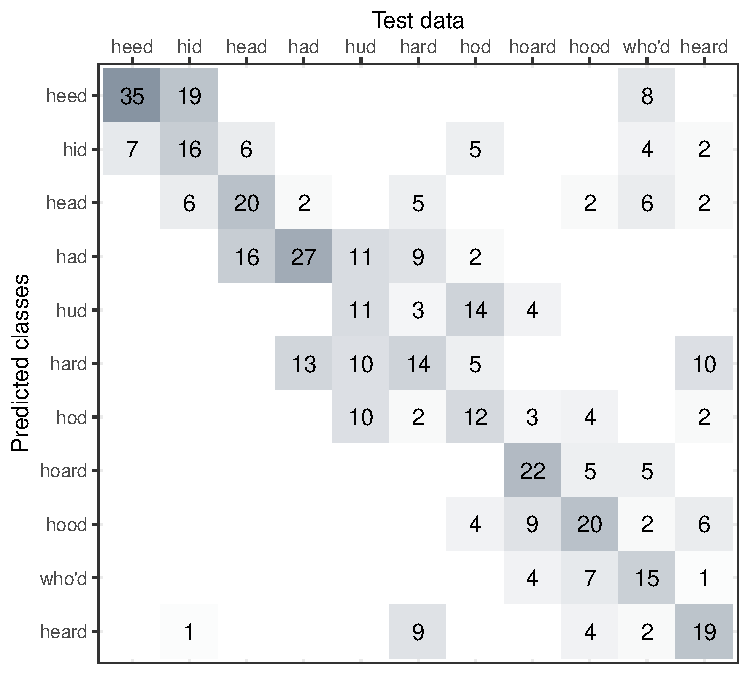
\includegraphics[width=0.485\linewidth]{figure/vowel_confusion_matrix-1} }
\subfloat[fBm-0.5 kernel\label{fig:vowel.confusion.matrix2}]{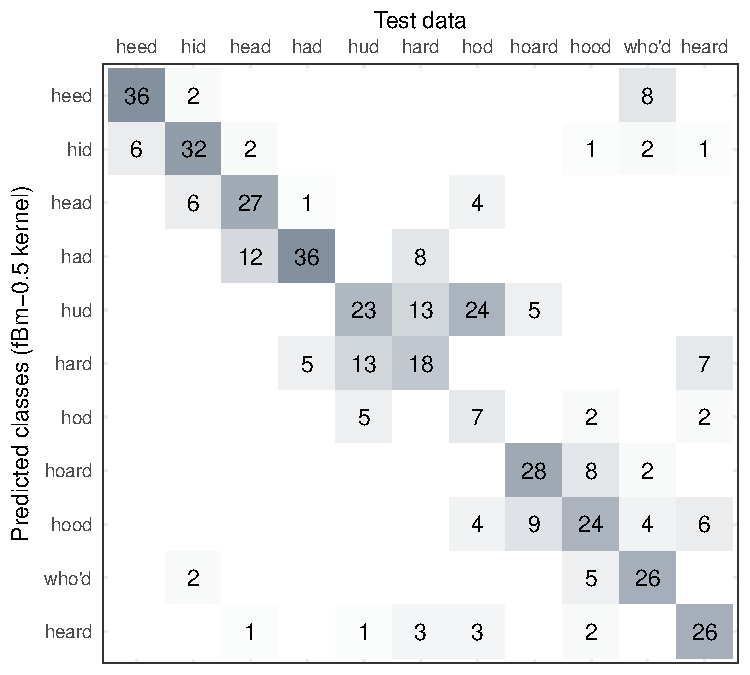
\includegraphics[width=0.485\linewidth]{figure/vowel_confusion_matrix-2} }

}

\caption[Confusion matrices for the vowel classification problem in which predicted values were obtained from the I-probit models]{Confusion matrices for the vowel classification problem in which predicted values were obtained from the I-probit models. The maximum value for any one cell is 42. Blank cells indicate nil values.}\label{fig:vowel.confusion.matrix}
\end{figure}


\end{knitrout}

A good way to visualise the performance of model predictions is through a confusion matrix, as shown in Figure \ref{fig:vowel.confusion.matrix}. The numbers in each row indicate the instances of a predicted class, while the numbers in the column indicate instances of the actual classes. Nil values are indicated by blank cells. A quick glance of the plots seem to favour the fBm-0.5 kernel as having better predictions. There are a lot more misclassifications when using the canonical kernel. Under the fBm-0.5 model, the model makes understandable mistakes - confusing very similar words, especially `hod' and `hud'.

Comparisons to other methods that had been used to analyse this data set is given in Table \ref{tab:vowel.tab}.
In particular, the I-probit model is compared against 1) linear regression; 2) logistic linear regression; 3) linear and quadratic discriminant analysis; 4) decision trees; 5) neural networks; 6) $k$-nearest neighbours; and 7) flexible discriminant analysis.
All of these methods are described in further detail in cite{Hastie Tibshirani}.
The I-probit model using the fBm-0.5 kernel offers one of the best out-of-sample classification error rates (38.7\%) of all the methods compared.
The linear I-probit model is seen to be comparable to logistic regression, linear and quadratic discrimant analysis, and also decision trees.
It also provides significant improvement over multiple linear regression.

\begin{knitrout}
\definecolor{shadecolor}{rgb}{1, 1, 1}\color{fgcolor}\begin{table}

\caption{\label{tab:vowel.tab}Results of various classification methods for the vowel data set.}
\centering
\begin{tabular}[t]{lrr}
\toprule
\multicolumn{1}{c}{ } & \multicolumn{2}{c}{Error rates} \\
\cmidrule(l{2pt}r{2pt}){2-3}
Method & Training & Test\\
\midrule
Linear regression & 48 & 67\\
Logistic regression & 22 & 51\\
Linear discriminant analysis & 32 & 56\\
Quadratic discriminant analysis & 1 & 53\\
\addlinespace
Decision trees & 5 & 54\\
Neural networks &  & 45\\
k-Nearest neighbours &  & 44\\
FDA/BRUTO & 6 & 44\\
FDA/MARS & 13 & 39\\
\addlinespace
I-probit (fBm-0.5) & 22 & 39\\
I-probit (linear) & 28 & 54\\
\bottomrule
\end{tabular}
\end{table}


\end{knitrout}

\end{document}




\section{Spatio-temporal modelling of bovine tubercolosis in Cornwall}
\documentclass[a4paper,showframe,11pt]{report}\usepackage[]{graphicx}\usepackage[]{color}
%% maxwidth is the original width if it is less than linewidth
%% otherwise use linewidth (to make sure the graphics do not exceed the margin)
\makeatletter
\def\maxwidth{ %
  \ifdim\Gin@nat@width>\linewidth
    \linewidth
  \else
    \Gin@nat@width
  \fi
}
\makeatother

\definecolor{fgcolor}{rgb}{0.196, 0.196, 0.196}
\newcommand{\hlnum}[1]{\textcolor[rgb]{0.063,0.58,0.627}{#1}}%
\newcommand{\hlstr}[1]{\textcolor[rgb]{0.063,0.58,0.627}{#1}}%
\newcommand{\hlcom}[1]{\textcolor[rgb]{0.588,0.588,0.588}{#1}}%
\newcommand{\hlopt}[1]{\textcolor[rgb]{0.196,0.196,0.196}{#1}}%
\newcommand{\hlstd}[1]{\textcolor[rgb]{0.196,0.196,0.196}{#1}}%
\newcommand{\hlkwa}[1]{\textcolor[rgb]{0.231,0.416,0.784}{#1}}%
\newcommand{\hlkwb}[1]{\textcolor[rgb]{0.627,0,0.314}{#1}}%
\newcommand{\hlkwc}[1]{\textcolor[rgb]{0,0.631,0.314}{#1}}%
\newcommand{\hlkwd}[1]{\textcolor[rgb]{0.78,0.227,0.412}{#1}}%
\let\hlipl\hlkwb

\usepackage{framed}
\makeatletter
\newenvironment{kframe}{%
 \def\at@end@of@kframe{}%
 \ifinner\ifhmode%
  \def\at@end@of@kframe{\end{minipage}}%
  \begin{minipage}{\columnwidth}%
 \fi\fi%
 \def\FrameCommand##1{\hskip\@totalleftmargin \hskip-\fboxsep
 \colorbox{shadecolor}{##1}\hskip-\fboxsep
     % There is no \\@totalrightmargin, so:
     \hskip-\linewidth \hskip-\@totalleftmargin \hskip\columnwidth}%
 \MakeFramed {\advance\hsize-\width
   \@totalleftmargin\z@ \linewidth\hsize
   \@setminipage}}%
 {\par\unskip\endMakeFramed%
 \at@end@of@kframe}
\makeatother

\definecolor{shadecolor}{rgb}{.97, .97, .97}
\definecolor{messagecolor}{rgb}{0, 0, 0}
\definecolor{warningcolor}{rgb}{1, 0, 1}
\definecolor{errorcolor}{rgb}{1, 0, 0}
\newenvironment{knitrout}{}{} % an empty environment to be redefined in TeX

\usepackage{alltt}
\usepackage{standalone}
\standalonetrue
\ifstandalone
  \usepackage{../../haziq_thesis}
  \usepackage{../../haziq_maths}
  \usepackage{../../haziq_glossary}
  \addbibresource{../../bib/haziq.bib}
  \externaldocument{../01/.texpadtmp/introduction}
\fi







\IfFileExists{upquote.sty}{\usepackage{upquote}}{}
\begin{document}

Data containing the number of breakdows of bovine tubercolosis (BTB) in Cornwall, the locations of the infected animals, and the year of occurence is analysed.
The interest, as motivated by veterinary epidimiology, is to understand whether or not there is spatial segregation between the herds, and whether there is a time-element to presence or absence of this spatial segregation.
There have been previous work done to analyse this data set: \hltodo{cite Diggle et al. (2005)} developed a non-parametric method to estimate spatial segregation using a multivariate point process.
The occurrences are modelled as Poisson point processes, and spatial segregation is said to have occured if the model-estimated type-specific breakdown probabilities at any given location are not significantly different from the sample proportions \hltodo{I think this is what they did - recheck}.
The authors estimated the probabilities via kernel regression, and the resulting test statistic had to be estimated via Monte Carlo methods.
Other work includes Taylor et al. (2015), who used a fully Bayes scheme for spatio-temporal multivariate log-Gaussian Cox processes.

\begin{knitrout}
\definecolor{shadecolor}{rgb}{1, 1, 1}\color{fgcolor}\begin{figure}[h]

{\centering 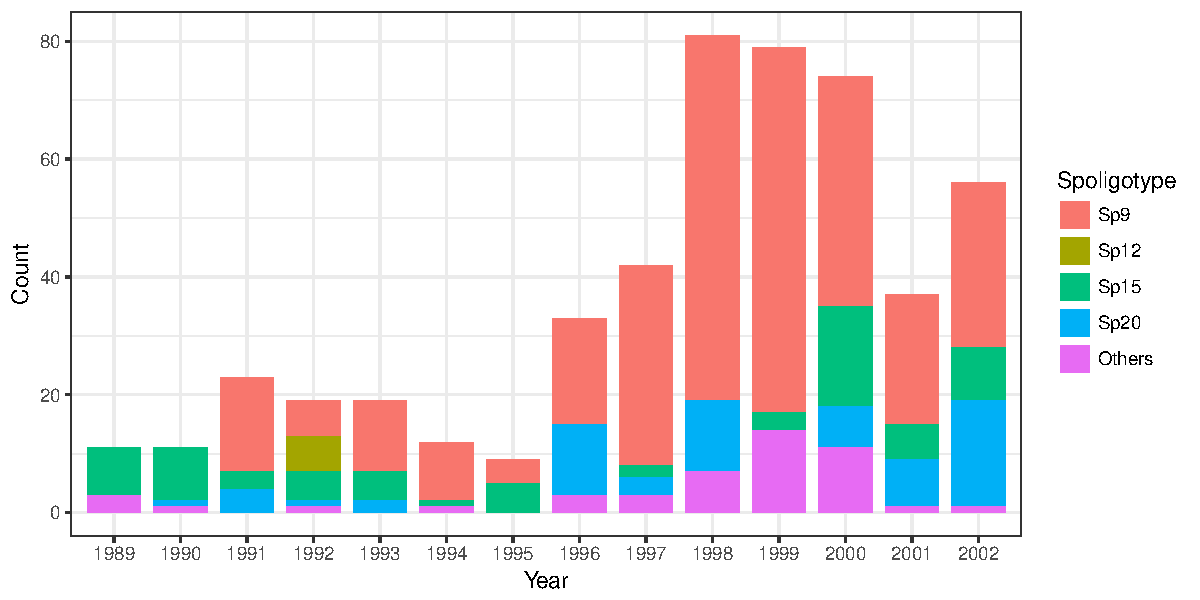
\includegraphics[width=\linewidth]{figure/plot_cow-1} 

}

\caption[Distribution of the different types (Spoligotypes) of bovine tubercolosis affecting herds in Cornwall over the period 1989 to 2002]{Distribution of the different types (Spoligotypes) of bovine tubercolosis affecting herds in Cornwall over the period 1989 to 2002.}\label{fig:plot.cow}
\end{figure}


\end{knitrout}

\hltodo{Explain data set}. $n=919$ cases in total. Originally there are 11 spoligotypes, but of these, four are most common. Therefore, the rest are combined into a separate class of `Others`. Total 14 years of data, so total number of classes is $m = 5$.

\begin{knitrout}
\definecolor{shadecolor}{rgb}{1, 1, 1}\color{fgcolor}\begin{figure}[h]

{\centering 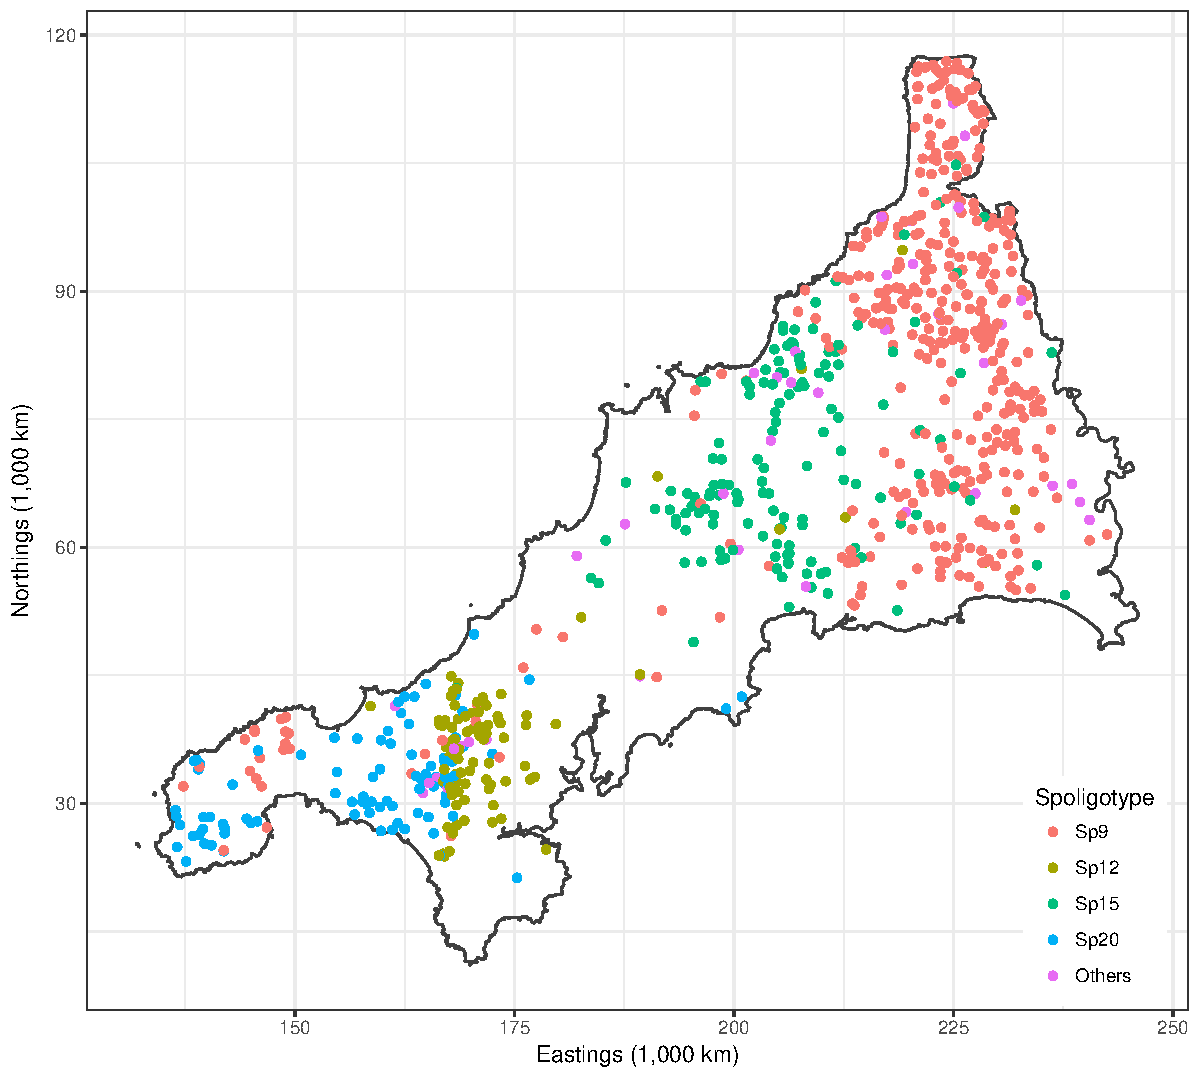
\includegraphics[width=\linewidth]{figure/plot_cornwall-1} 

}

\caption[Spatial distribution of all cases over the 14 years]{Spatial distribution of all cases over the 14 years.}\label{fig:plot.cornwall}
\end{figure}


\end{knitrout}

We are able to investigate any spatio-temporal patterns of infection using I-priors rather simply.
Let $p_{ij}$ denote the probability that a particular animal $i$ is infected with the disease with spoligotype $j \in \{1,\dots,m\}$.
We model the transformed probabilities $g(p_{ij})$ (as described in the categorical response chapter) as following a smooth function $f$ which takes two covariates: the spatial data $x_1$ (Northings and Eastings, measured in kilometres), and the temporal data $x_2$ (year of infection):
\begin{align*}
  g(p_{ij}) &= f_j(x_1, x_2) \\
  &= f_{1j}(x_1) + f_{2j}(x_2) + f_{12j}(x_1, x_2)
\end{align*}
We assume a smooth effect of space and time on the probabilities, and an appropriate RKHS for the functions $f_1$ and $f_2$ are the fBm-0.5 RKHS. Alternatively, as per Diggle et al., divide the data into four distinct time periods: 1) 1996 and earlier; 2) 1997 to 1998; 3) 1999 to 2000; and finally 4) 2001 to 2002. In this case, $x_2$ would indicate which period the infection took place in, and thus would have a nominal effect on the probabilities. An appropriate RKHS for $f_2$ in such a case would be the Pearson RKHS. In either case, the function $f_{12}$ would be the ``interaction effect'', meaning that with such an effect present, the spatial distribution of the diseases are assumed to vary across the years.

Let $h_k$, $k \in \{1,2\}$ denote the reproducing kernel of the spatial and temporal RKHSs respectively.
Then, an I-prior on $f_j$ takes the form
\begin{align*}
  f_j(x_1, x_2) &= \lambda_{1j} \sum_{i=1}^n h_1(x_1, x_{i1}) w_{ij} +
  \lambda_{2j} \sum_{i=1}^n h_2(x_2, x_{i2}) w_{ij} \\
  &\phantom{==} + \lambda_{1j} \lambda_{2j} \sum_{i=1}^n  h_1(x_1, x_{i1})h_2(x_2, x_{i2}) w_{ij}
\end{align*}
where $\bw_j = (w_{1j}, \dots, w_{nj})^\top \sim \N(0,\bI_n)$ and each of the $\bw_j$ are also independent of each other.
The parameters $\lambda_{1j}$ and $\lambda_{2j}$ are the RKHS scale parameters for the spatial and temporal covariates respectively.
Notice that the functions are indexed by the classes $j$, such that there would be $2m$ scale parameters to estimate.
This is the more general case, in which we assume \emph{separate scale} parameters in each class.
However, we may also restrict the scale parameters to be equivalent in each class, so that this so-called \emph{shared scale} model has only two parameters to estimate, which is simpler to do inference.
Note that there are also intercept parameters to estimate (one in each class), but these will not be reported as they are irrelevant to the discussion at hand.

Spatio-temporal effects of the BTB breakdowns can be easily inferred through the RKHS scale parameters.
The hypothesis of temporal significance is the same as testing the significance of the $\lambda_2$ parameter, while the test of both spatial and temporal effects are conducted on $\lambda_1$ and $\lambda_2$ simultaneously (equivalent to modelling $f$ with a constant).
For these tests, it is simpler to infer from the shared scale model, for which we can read the results directly of off Table \ref{tab:table.btb}.
The said table displays the posterior mean estimate of the scale parameters, and together with its posterior standard deviation.
From Chapter X, we know that these scale parameters follow a normal posterior distribution, so we can calculate the $Z$-scores by dividing the mean by its corresponding s.d..
Absolute values greater than three would satisfy a Bayesian hypothesis test of significance at the 0.01 level, for which we see all parameters satisfy in the shared scale model.


\begin{landscape}\begin{table}

\caption{\label{tab:table.btb}Results of the fitted I-probit models.}
\centering
\begin{tabular}[t]{lrrrlrrrlrrrl}
\toprule
\multicolumn{ 1}{c}{\bfseries  } & \multicolumn{12}{c}{\bfseries Model} \\
\cmidrule(l{2pt}r{2pt}){2-13}
\multicolumn{1}{c}{ } & \multicolumn{3}{c}{Spatial} & \multicolumn{1}{c}{ } & \multicolumn{3}{c}{Spatio-temporal} & \multicolumn{1}{c}{ } & \multicolumn{3}{c}{Spatio-period} \\
\cmidrule(l{2pt}r{2pt}){2-4} \cmidrule(l{2pt}r{2pt}){6-8} \cmidrule(l{2pt}r{2pt}){10-12}
  & Estimate & S.D. & |$Z$|-score &  & Estimate & S.D. & |$Z$|-score &  & Estimate & S.D. & |$Z$|-score & \\
\midrule
\addlinespace[0.5em]
\multicolumn{13}{l}{\textbf{Shared scale model}}\\
\hspace{1em}Spatial & 0.19 & 0.003 & 64.9 & *** & 0.18 & 0.003 & 67.4 & *** & 0.19 & 0.003 & 65.6 & ***\\
\hspace{1em}Temporal &  &  &  &  & 0.01 & 0.000 & 16.5 & *** & 0.00 & 0.000 & 12.0 & ***\\
\addlinespace[0.5em]
\multicolumn{13}{l}{\textbf{Separate scale model}}\\
\hspace{1em}Spatial (Sp9) & 0.47 & 0.014 & 33.5 & *** & 0.48 & 0.014 & 33.1 & *** & 0.47 & 0.014 & 33.9 & ***\\
\hspace{1em}Spatial (Sp12) & 0.19 & 0.007 & 29.2 & *** & 0.26 & 0.008 & 31.4 & *** & 0.23 & 0.007 & 31.3 & ***\\
\hspace{1em}Spatial (Sp15) & 0.17 & 0.005 & 33.9 & *** & 0.17 & 0.005 & 33.6 & *** & 0.17 & 0.005 & 33.9 & ***\\
\hspace{1em}Spatial (Sp20) & 0.16 & 0.004 & 44.2 & *** & 0.17 & 0.004 & 39.6 & *** & 0.17 & 0.004 & 40.7 & ***\\
\hspace{1em}Spatial (Others) & 0.00 & 0.004 & 0.0 &  & 0.00 & 0.004 & 0.0 &  & 0.00 & 0.004 & 0.0 & \\
\hspace{1em}Temporal (Sp9) &  &  &  &  & 0.00 & 0.002 & 0.1 &  & 0.00 & 0.001 & 6.3 & ***\\
\hspace{1em}Temporal (Sp12) &  &  &  &  & 0.01 & 0.001 & 17.8 & *** & 0.01 & 0.001 & 12.4 & ***\\
\hspace{1em}Temporal (Sp15) &  &  &  &  & 0.02 & 0.001 & 12.3 & *** & 0.00 & 0.001 & 0.0 & \\
\hspace{1em}Temporal (Sp20) &  &  &  &  & 0.00 & 0.002 & 0.1 &  & 0.00 & 0.001 & 0.1 & \\
\hspace{1em}Temporal (Others) &  &  &  &  & 0.00 & 0.002 & 0.0 &  & 0.01 & 0.001 & 10.9 & ***\\
\bottomrule
\multicolumn{13}{l}{\textsuperscript{*} Lower-bound values (Brier scores) for the shared scale model are -664.8 (0.143), -654.9 (0.135), and -663.7 (0.136) respectively.}\\
\multicolumn{13}{l}{\textsuperscript{\dag} Lower-bound values (Brier scores) for the separate scale model are -660.8 (0.138), -667.9 (0.129), and -678.3 (0.130) respectively.}\\
\end{tabular}
\end{table}
\end{landscape}



A similar conclusion is reached when inferring from the separate scale model. Instead of individual tests of significance, we now need to test
\[
  \text{H}_0: \lambda_1 = \dots = \lambda_m = 0.
\]

We know that by the mean-field approximation used, the $\lambda_j$s are independent of each other, and therefore a $\chi^2$ test statistic can be built via
\[
  \chi^2 = \sum_{j=1}^m Z_j^2
\]
which is then compared against extreme values of the $\chi^2_m$-distribution.
As is often the case, separate scale models tend to fit the data better as it gives more generality due to having different scale parameters in each class.
This is also the case for the BTB data, where we see from the footnotes of Table \ref{tab:table.btb} that the Brier scores for the separate scale models are better than the Brier scores in the shared scale models.
For all following plots, we made use of the separate scale model for predicting the surface probabilities. Another comment regarding the models is that the conclusion remains the same if we had used the periodic formulation for $x_2$.

\begin{knitrout}
\definecolor{shadecolor}{rgb}{1, 1, 1}\color{fgcolor}\begin{figure}[h]

{\centering 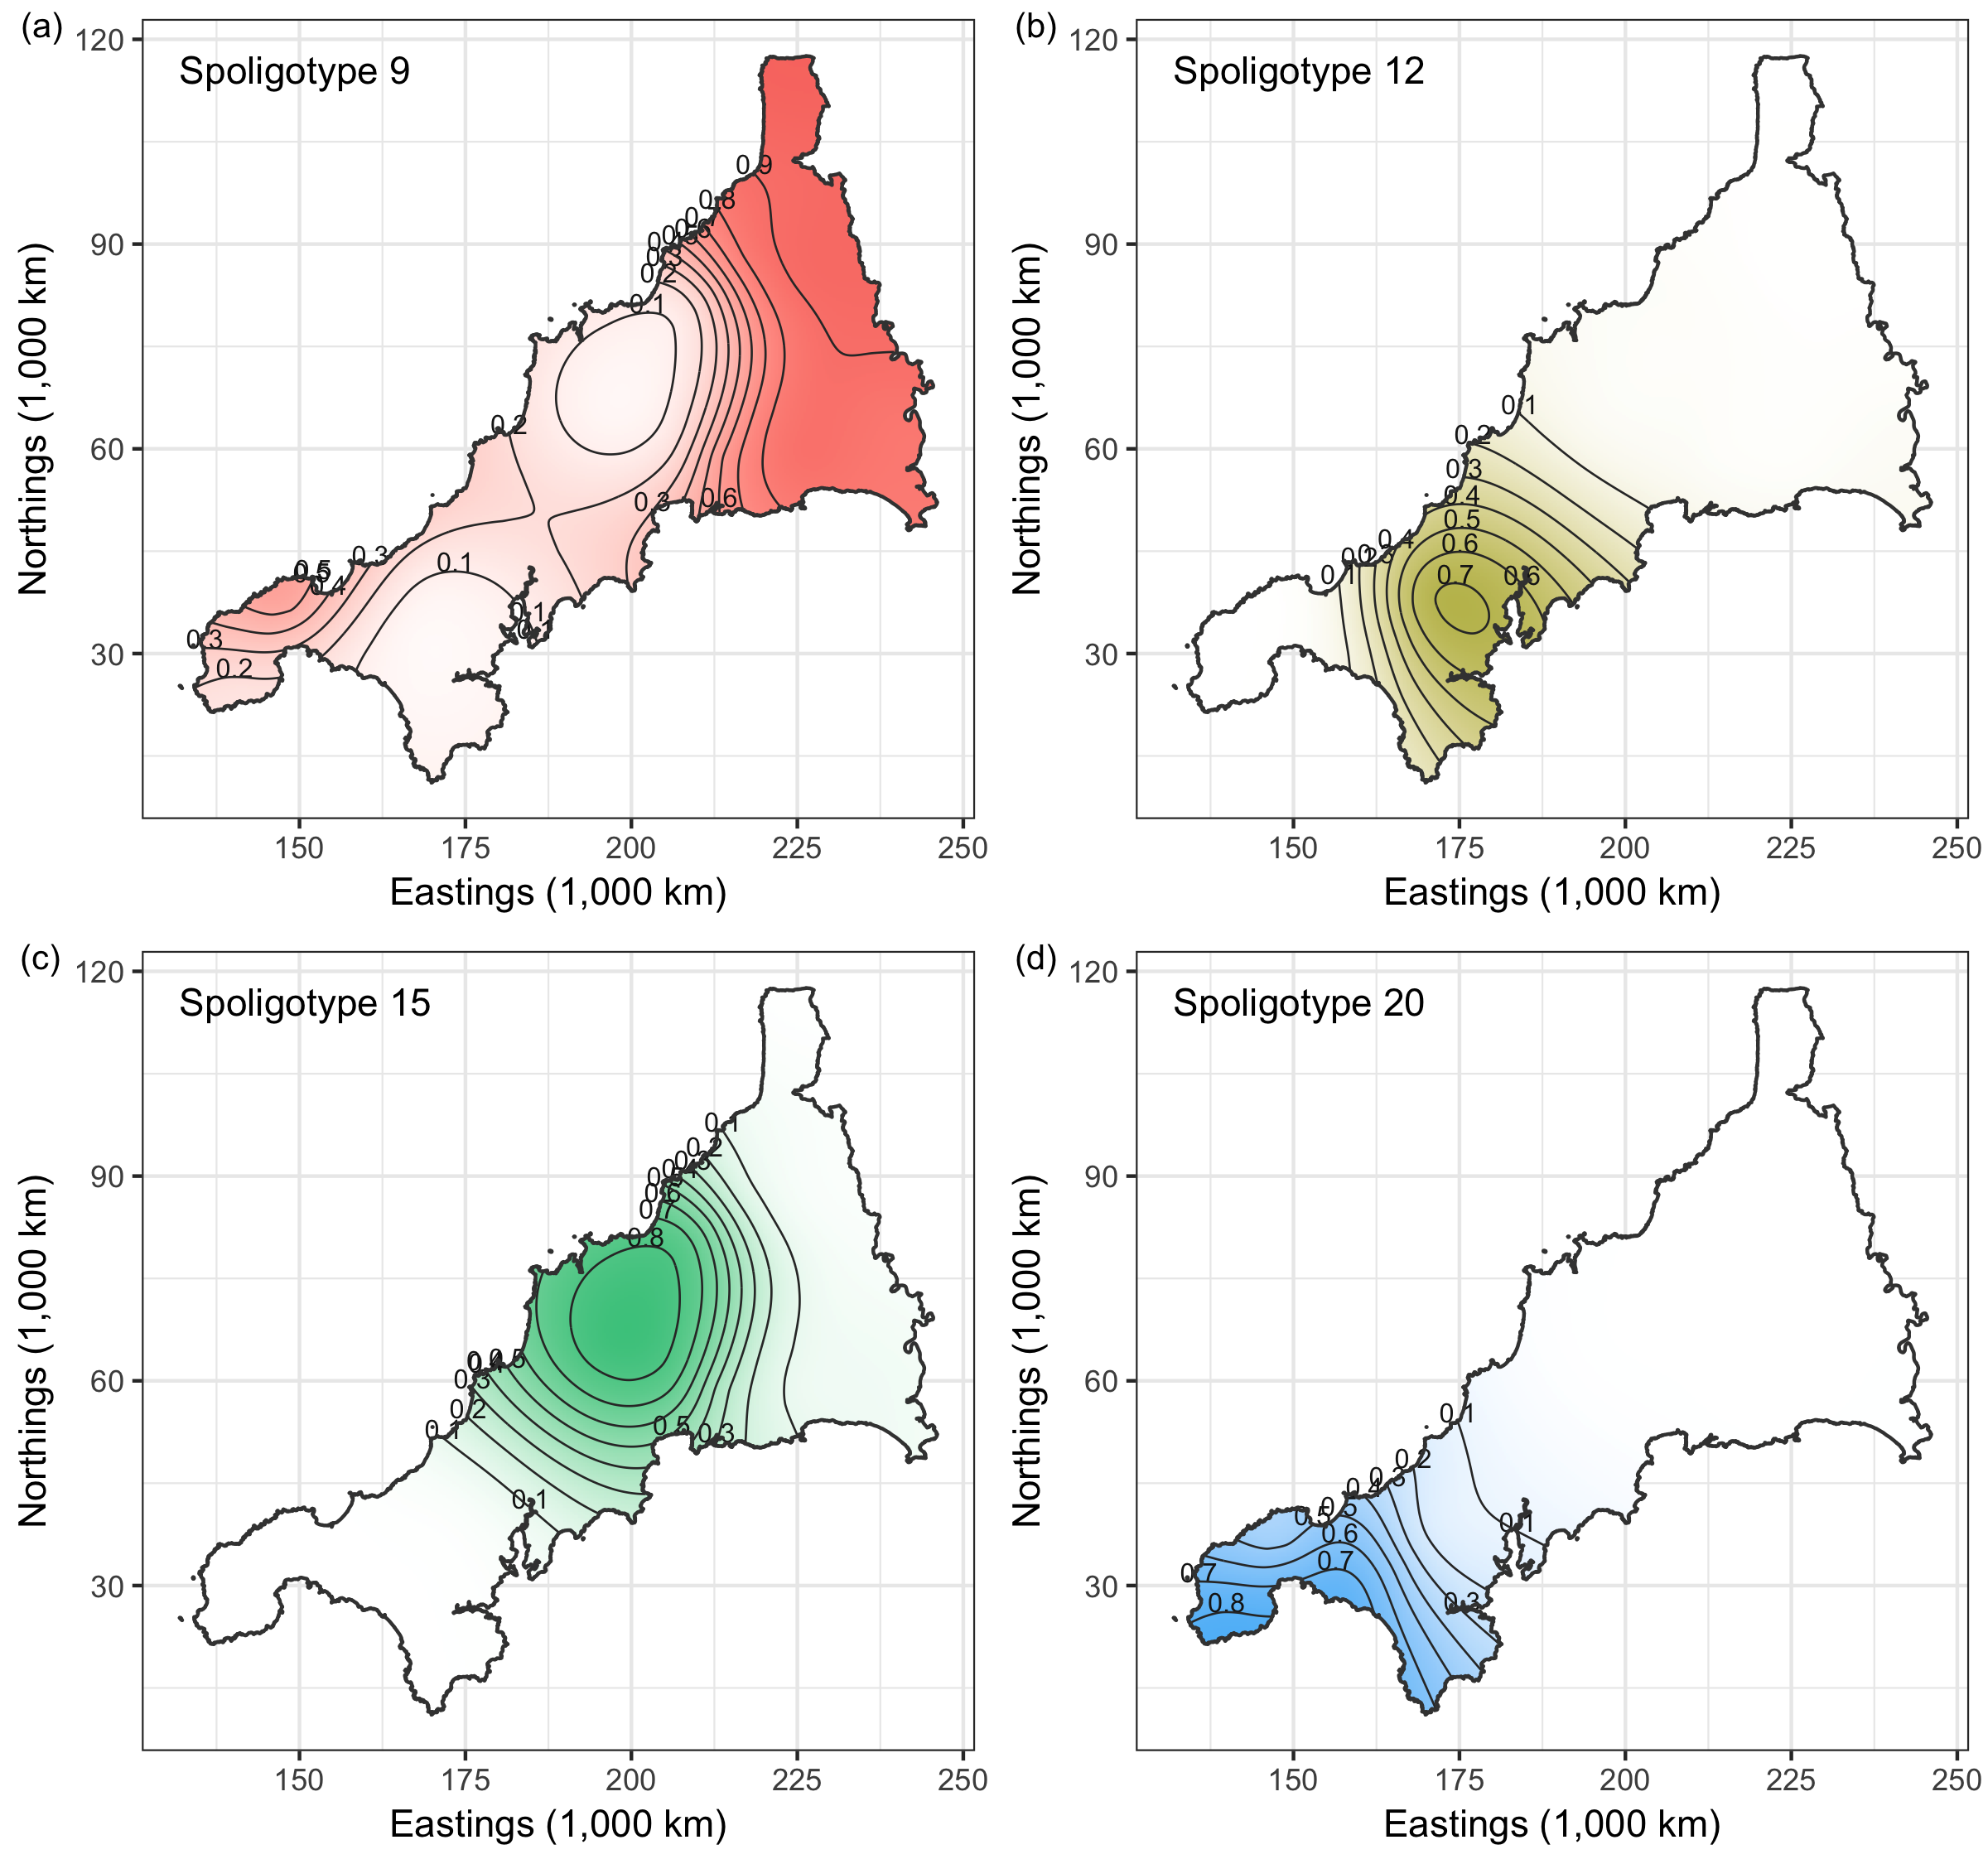
\includegraphics[width=\linewidth]{figure/plot_btb-1} 

}

\caption[Caption]{Caption.}\label{fig:plot.btb}
\end{figure}


\end{knitrout}

For a more visual approach, we can look at the plots of the surface probabilities.
To obtain these probabilities, we first determined the spatial points (Northings and Eastings) which fall inside the polygon which makes up Cornwall.
We then obtained predicted probabilities for each class of disease at each location.
Figure \ref{fig:plot.btb} was obtained using the model with spatial covariates only, thus ignoring any temporal effects.
In the case of the spatio-temporal model, we used the model which had the period formulation for time.
This way, we can obtain the surface probabilities in only four time periods, although there is no issue with using the continuous time model.
It is more economical to display four plots rather than the 14 yearly plots within the margins of this thesis.

As the model suggests, there is indeed spatial segregation for the four most common spoligotypes, and this is also very prominently seen from Figure \ref{fig:plot.btb}.
In comparing the distribution of the spoligotypes over the years, we may refer to Figure \ref{fig:plot.temporal.btb}.
For each time period, we superimpose the actual observations onto the predicted surface probabilities.
In addition, coloured dotted lines are displayed to indicate the ``decision boundaries'' for each of the four spoligotypes.
The most evident change is seen to the spatial distribution of spoligotype 12, with the decision boundary giving it a large area in years 1996 and earlier, but this steadily shrunk over the years.
Spoligotype 9, which is most commonly seen in the east of Cornwall, seems to have made its way down to the south-west over the years.
The other two spoligotypes seem to be rather constant over the years.
This is supported also by the spatio-period model results in Table \ref{tab:table.btb}, where the test of nullity for the scale parameters of these two spoligotypes are not rejected.

\begin{knitrout}
\definecolor{shadecolor}{rgb}{1, 1, 1}\color{fgcolor}\begin{figure}[h]

{\centering 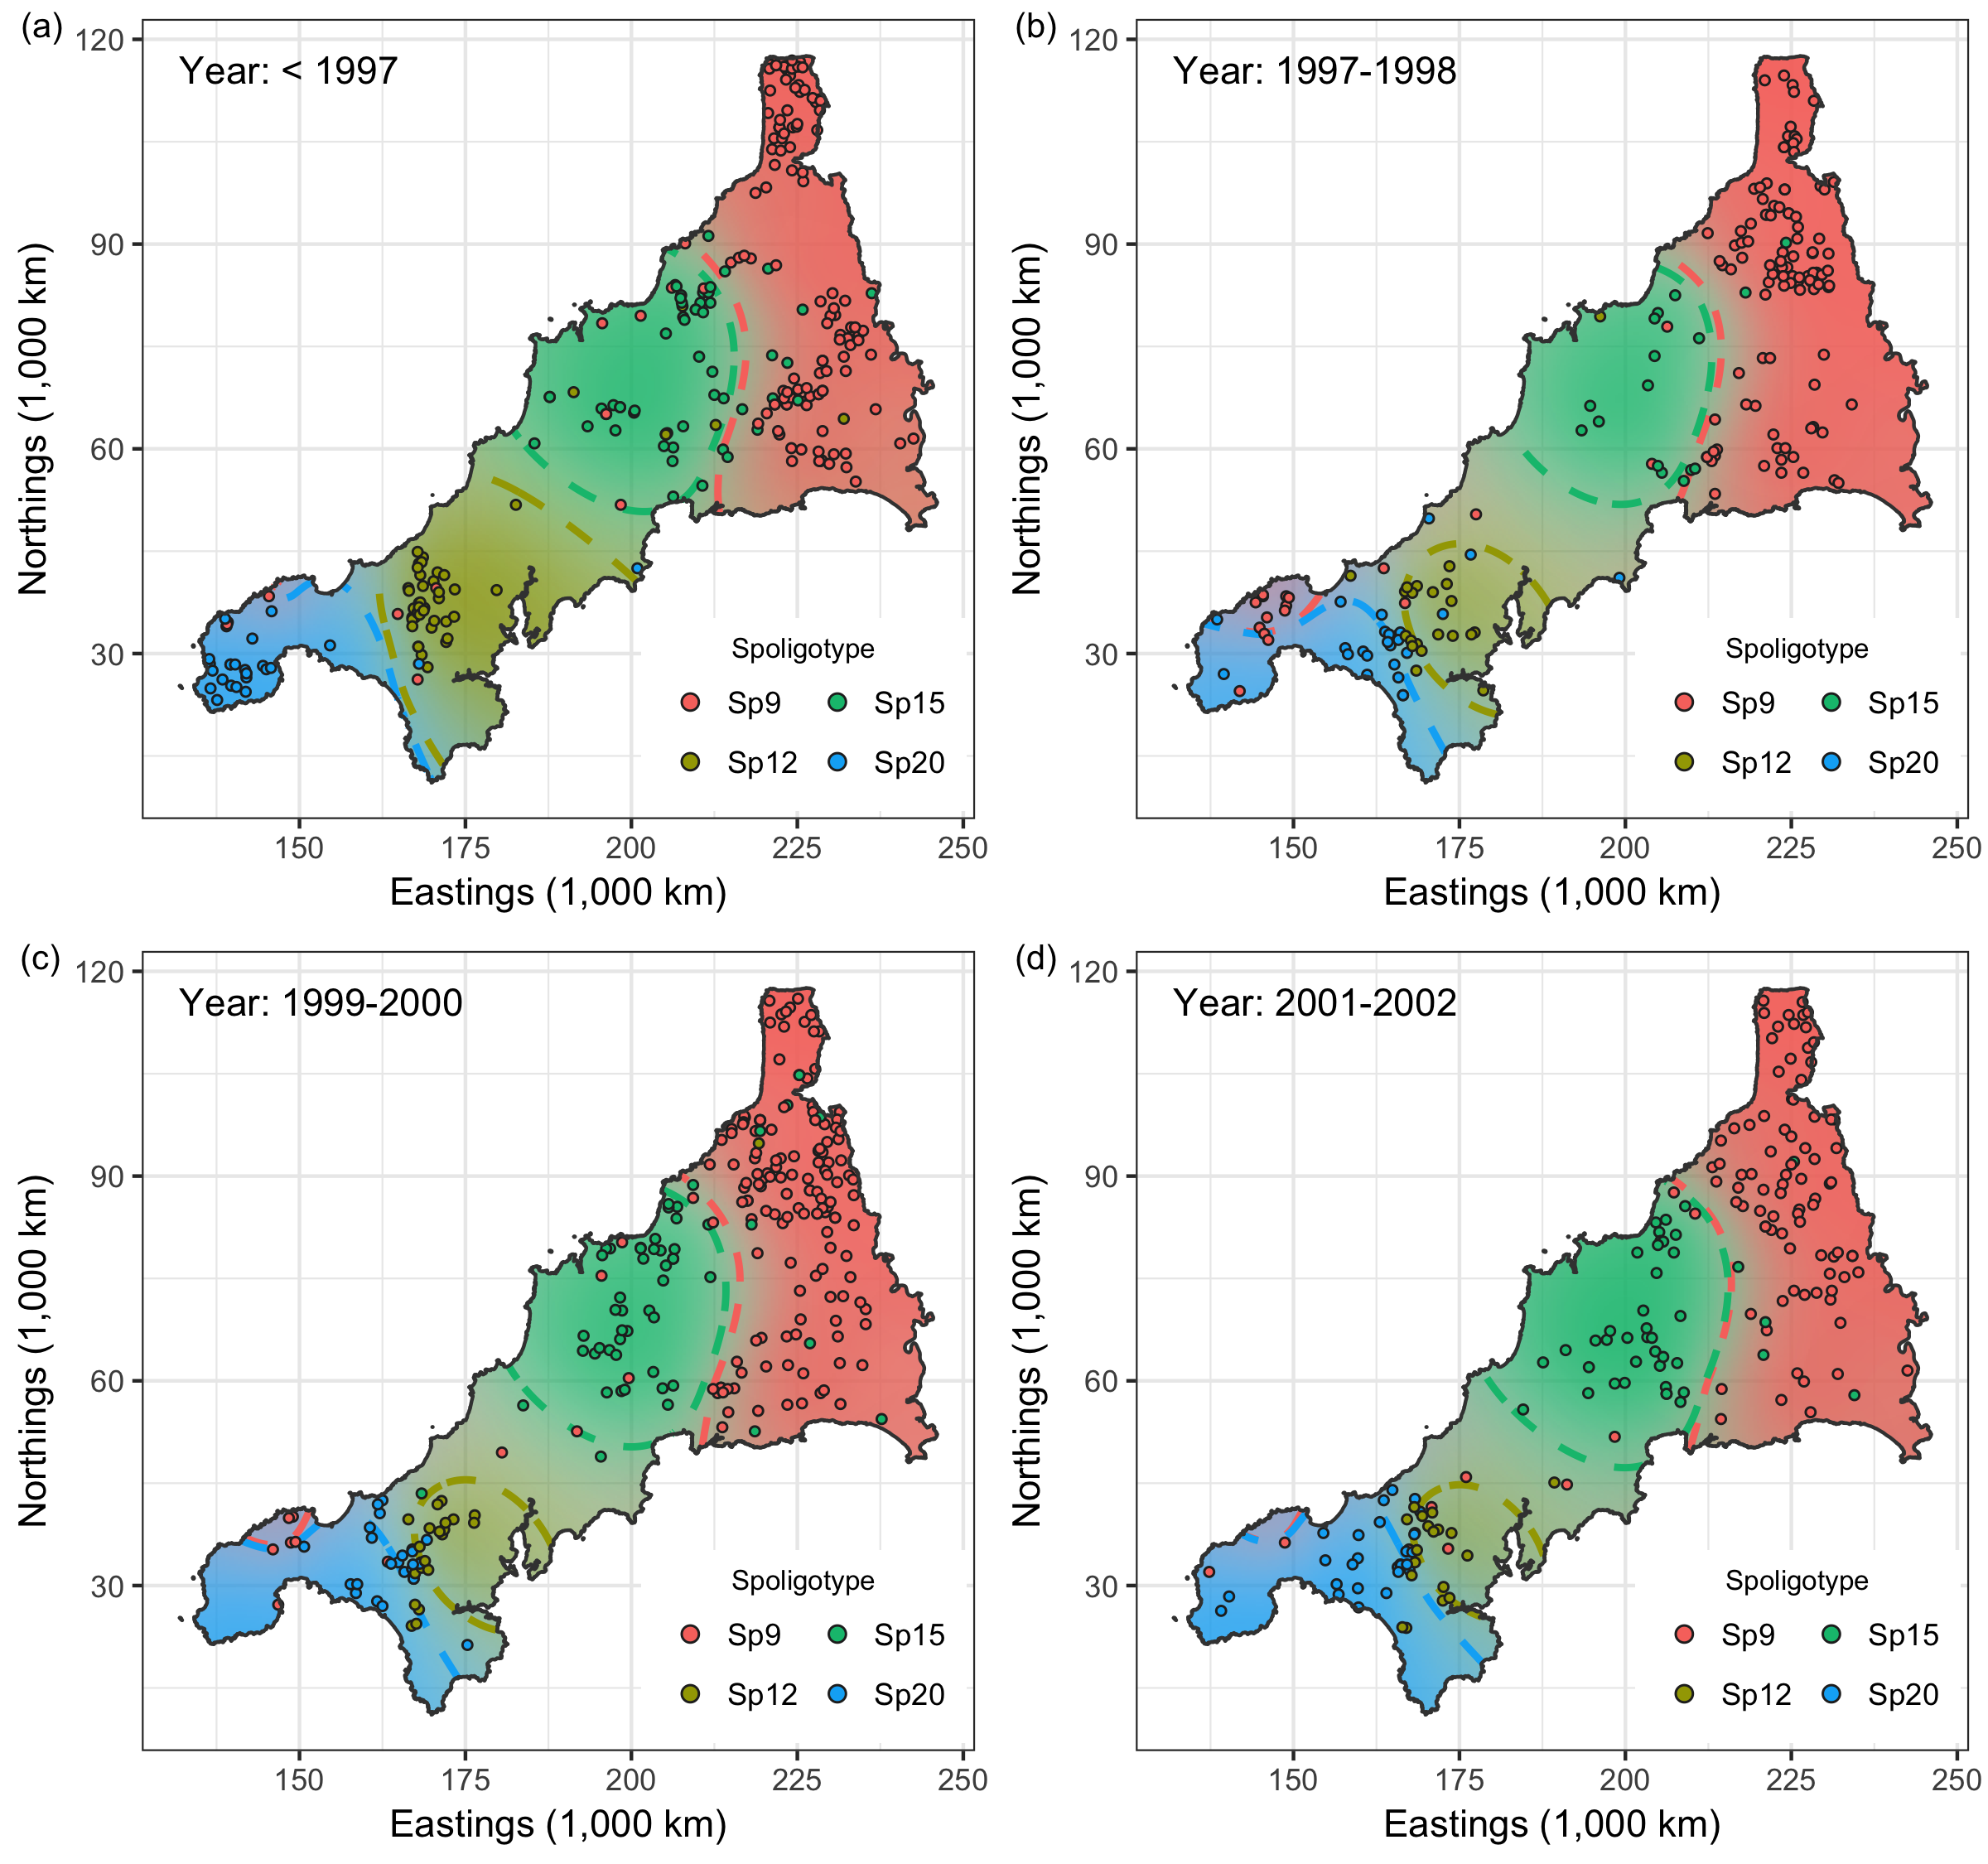
\includegraphics[width=\linewidth]{figure/plot_temporal_btb-1} 

}

\caption[Caption]{Caption.}\label{fig:plot.temporal.btb}
\end{figure}


\end{knitrout}

\end{document}




\section{Multi-class multivariate longitudinal data} 

Classification of psychotropic drugs based on EEG data (brain activity) of rats experiment. It is a longitudinal problem because the effect of the drugs are over a period of time in which the drug is in the system.

\hltodo{I would love to analyse this, but can't find the data set! Tempted to just create simulated data to back analyse, just as a proof of concept.}

\url{http://onlinelibrary.wiley.com/doi/10.1111/j.1467-9876.2007.00575.x/abstract}           

\hClosingStuffStandalone
\end{document}
